% =====================================================================
%  Figure captions for the eight validation panels of
%  "The Causal Propagation Table"
%  Include with % =====================================================================
%  Figure captions for the eight validation panels of
%  "The Causal Propagation Table"
%  Include with % =====================================================================
%  Figure captions for the eight validation panels of
%  "The Causal Propagation Table"
%  Include with % =====================================================================
%  Figure captions for the eight validation panels of
%  "The Causal Propagation Table"
%  Include with \input{figures/causal-captions} or copy individually.
% =====================================================================

% ---------------------------------------------------------------------
\begin{figure*}[!htbp]
    \centering
    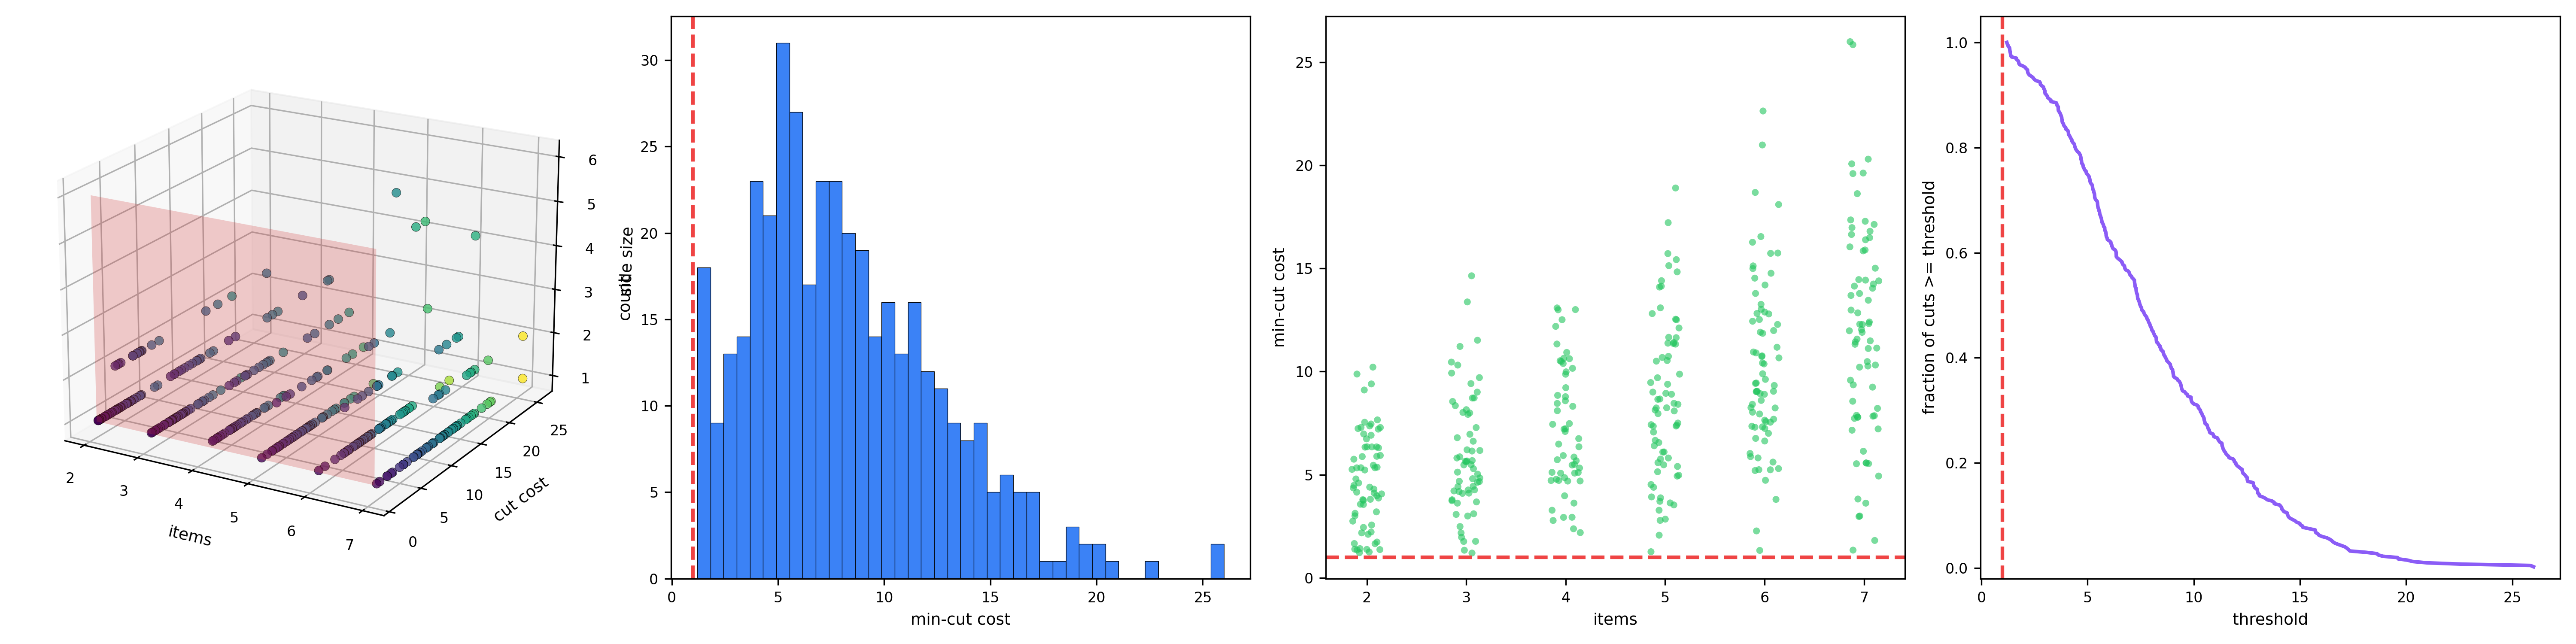
\includegraphics[width=\textwidth]{figures/panel_1_floor.png}
    \caption{\textbf{The Floor: Minimum Cuts over Random Contact Graphs.}
    (\textbf{A})~Three-dimensional scatter of $400$ random contact graphs in (number of items, minimum-cut cost, cut-side size) space, points coloured by cut cost (viridis), with the floor plane at cost $\beta$ drawn in red. Every point lies on or above the floor plane: no item is separated from the medium for less than $\beta$ (Theorem~\ref{thm:floor}).
    (\textbf{B})~Distribution of the exact minimum-cut costs (\texttt{networkx} max-flow) across the $400$ graphs, with the floor $\beta$ marked (red dashed). No mass falls below $\beta$, the absence of any sharp cut (Corollary~\ref{cor:no-sharp}).
    (\textbf{C})~Minimum-cut cost versus number of items (jittered) for all graphs; the entire cloud sits above the floor line $\beta$ (red dashed) independently of graph order, confirming the bound holds at every size.
    (\textbf{D})~Survival curve: the fraction of cuts with cost at least a given threshold, dropping from one only after the threshold passes $\beta$ (red dashed). The fraction at or above $\beta$ is unity---every one of the $300$ validated cuts clears the floor.}
    \label{fig:panel_floor}
\end{figure*}

% ---------------------------------------------------------------------
\begin{figure*}[!htbp]
    \centering
    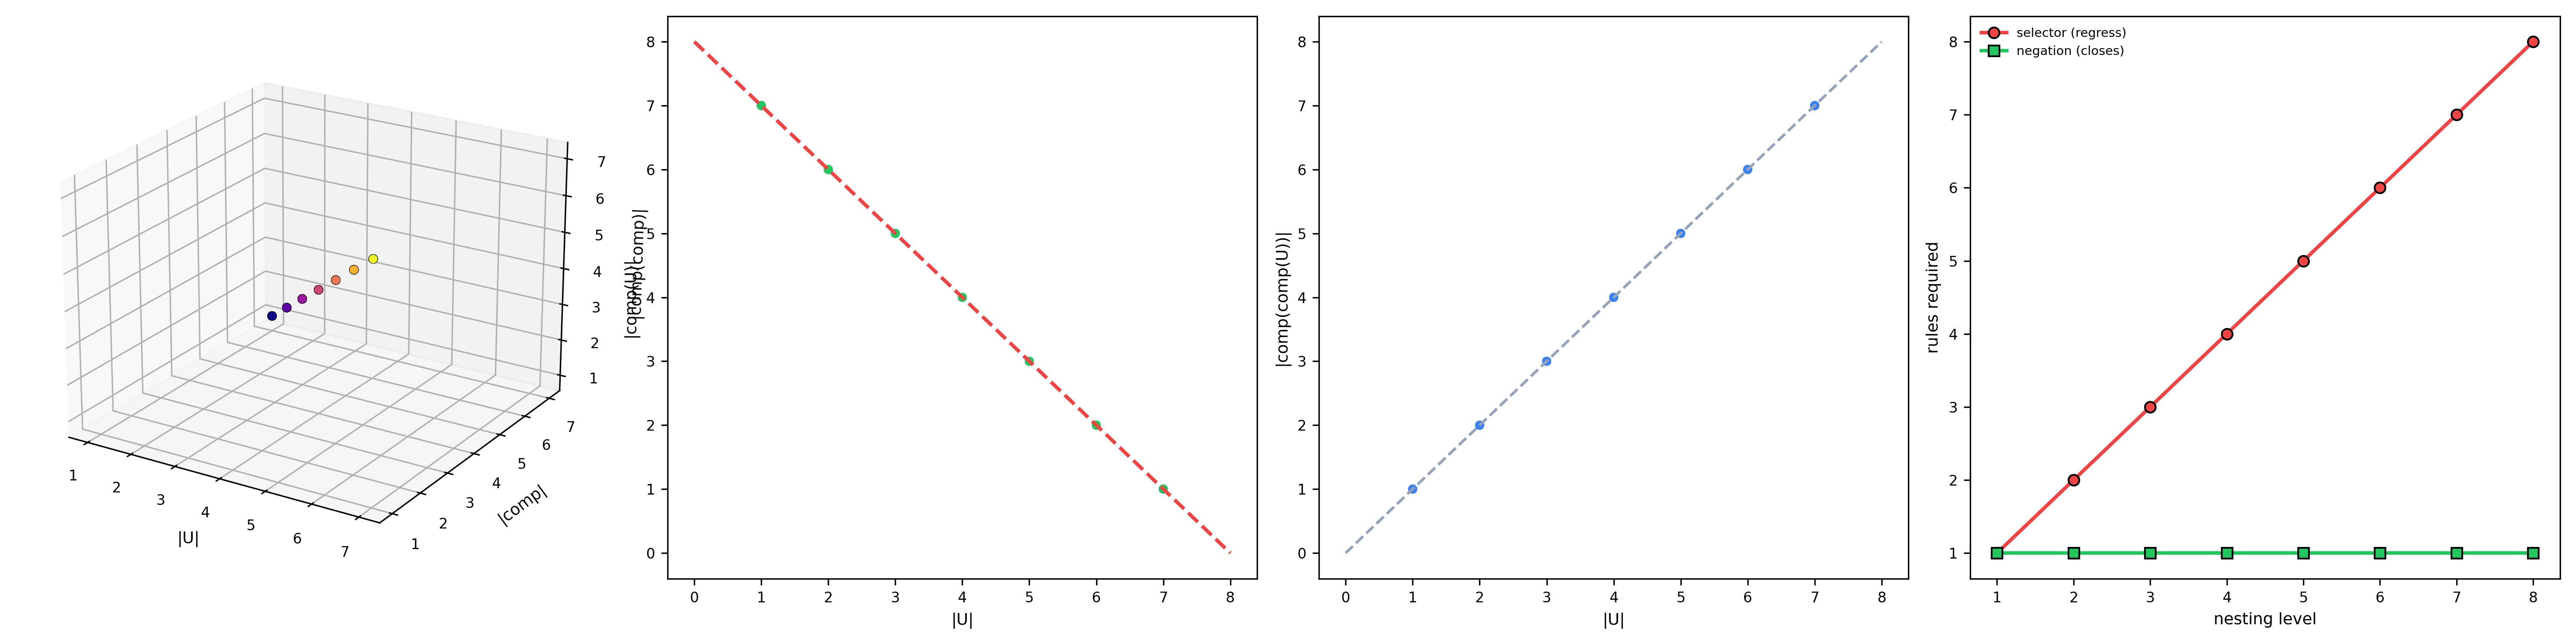
\includegraphics[width=\textwidth]{figures/panel_2_negation.png}
    \caption{\textbf{Individuation by Negation: the Complement Involution.}
    (\textbf{A})~Three-dimensional scatter of $200$ random subsets of an eight-element whole in $(|U|,\,|\co U|,\,|\co\co U|)$ space, coloured by $|U|$ (plasma). Every point satisfies $|\co\co U|=|U|$: double complementation returns the part, the involution underlying Theorem~\ref{thm:negation}.
    (\textbf{B})~Subset size $|U|$ versus complement size $|\co U|$; all points lie on the conservation line $|U|+|\co U|=8$ (red dashed): the complement is exactly ``the rest,'' fixed once the whole is given.
    (\textbf{C})~Double-complement size $|\co\co U|$ versus $|U|$ on the identity diagonal (grey dashed); the points coincide with the diagonal, so $\co$ is its own inverse and $\co U$ determines $U$ uniquely.
    (\textbf{D})~Rules required to fix a part as a function of nesting level: a positive (selector-based) rule regresses without bound (red), while negation closes at level one (green). The diverging red curve is the selector regress that Theorem~\ref{thm:negation} excludes; the flat green line is complementation, which needs only the whole.}
    \label{fig:panel_negation}
\end{figure*}

% ---------------------------------------------------------------------
\begin{figure*}[!htbp]
    \centering
    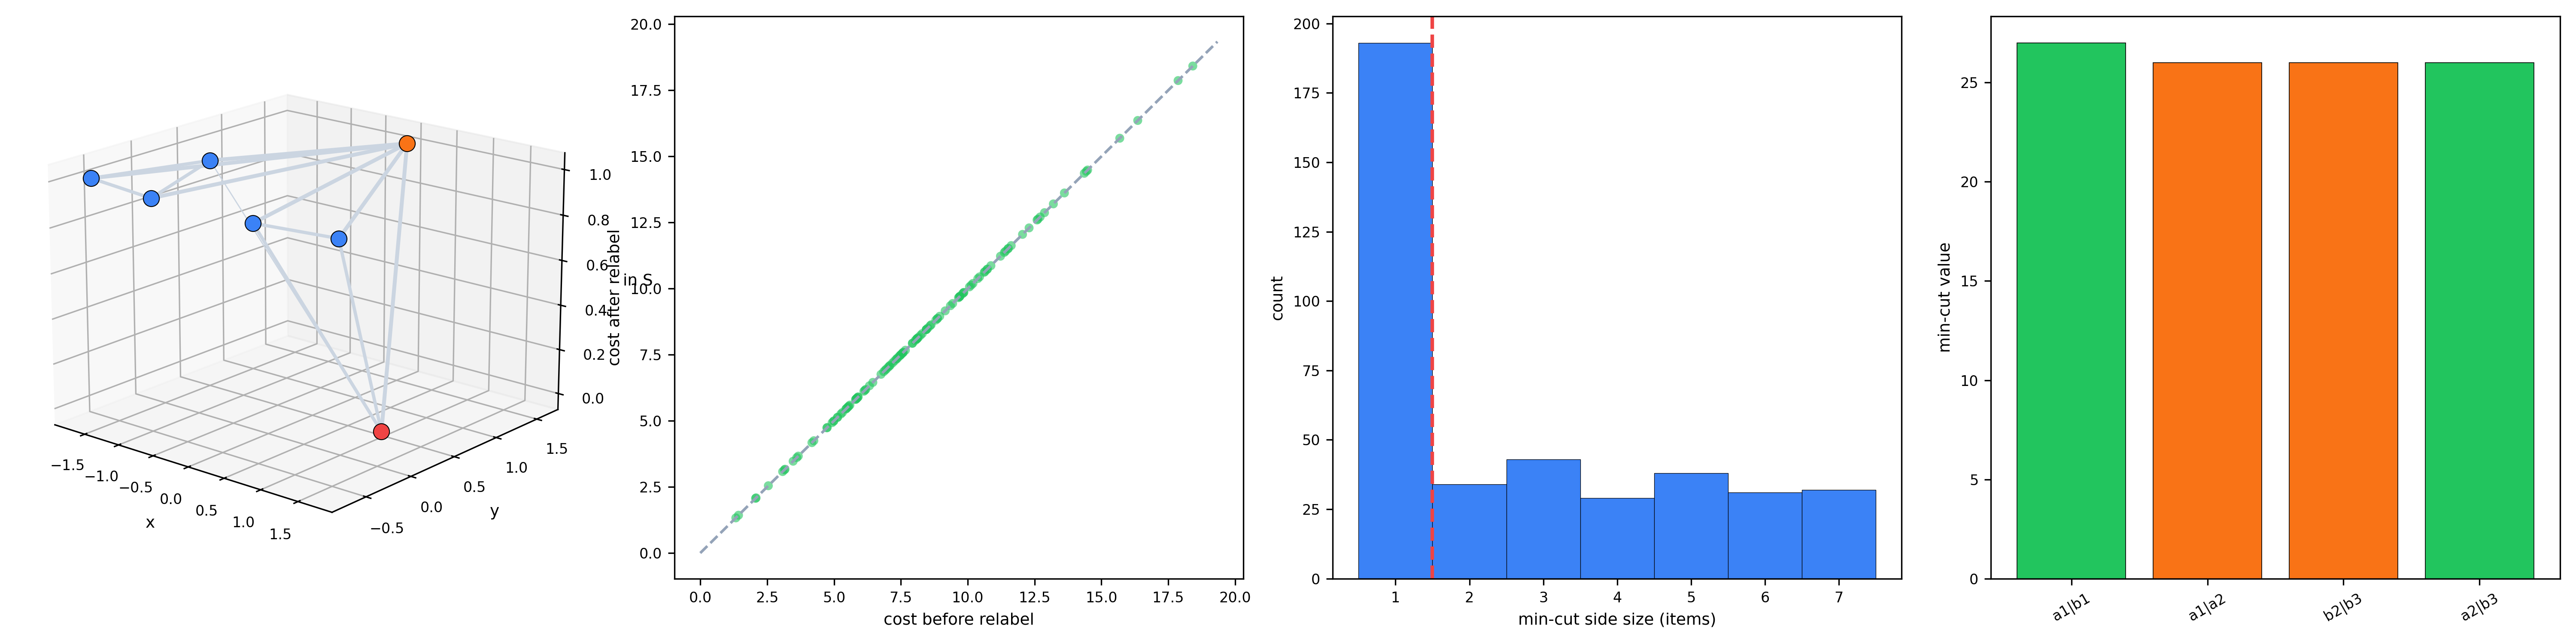
\includegraphics[width=\textwidth]{figures/panel_3_identity.png}
    \caption{\textbf{Identity as an Invariant Region, Never a Point.}
    (\textbf{A})~Three-dimensional rendering of the two-cluster contact graph: items (blue if on the source side $S$ of the minimum cut, red otherwise) and the medium (orange) at the origin, lifted on the vertical axis by cut membership, with edges drawn at width proportional to weight. The minimum cut places a multi-item set on the source side---identity is borne by a region, not a single vertex.
    (\textbf{B})~Minimum-cut cost before versus after a random relabelling (weighted isomorphism) of the items, over $120$ graphs; all points lie on the identity diagonal (grey dashed), so the cost is label-independent (Theorem~\ref{thm:invariant}).
    (\textbf{C})~Distribution of minimum-cut side sizes over $400$ random graphs; the mass lies predominantly above one item (the threshold at $1.5$, red dashed), the empirical content of ``the minimising side is in general not a singleton'' (Theorem~\ref{thm:region}).
    (\textbf{D})~Minimum-cut value for four different separated pairs in the two-cluster instance: the cluster-separating pairs (green) realise the cheap inter-cluster cut, while same-cluster pairs (orange) cost more, showing the cut value is a property of the partition, not of a chosen endpoint.}
    \label{fig:panel_identity}
\end{figure*}

% ---------------------------------------------------------------------
\begin{figure*}[!htbp]
    \centering
    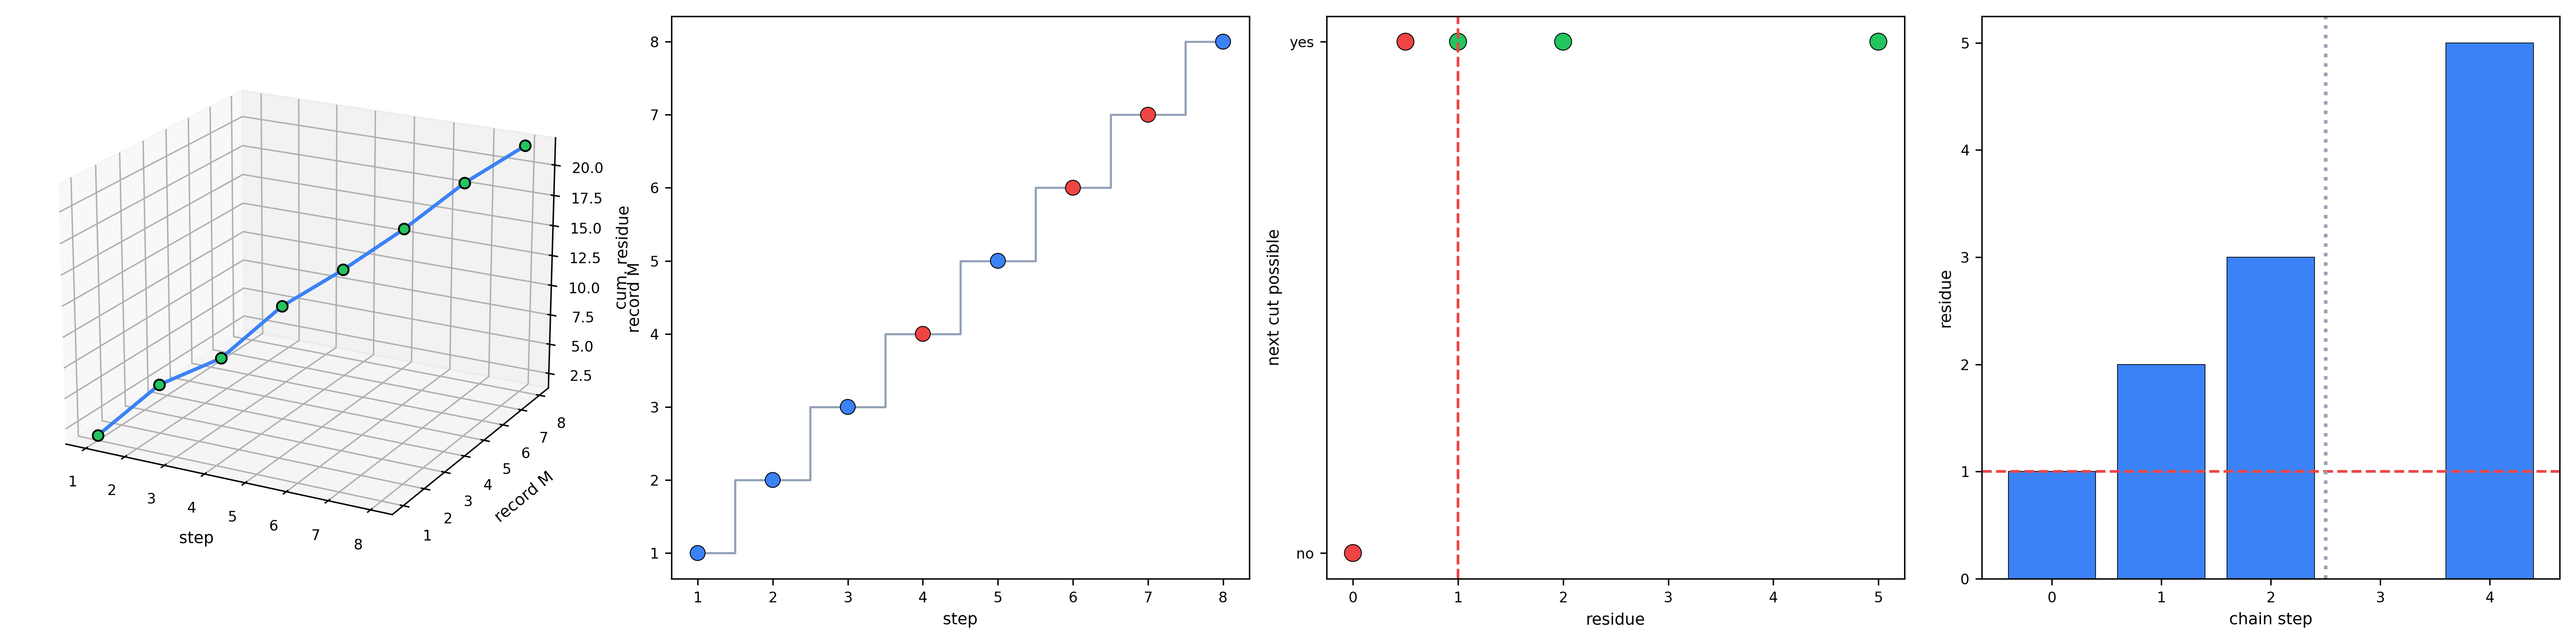
\includegraphics[width=\textwidth]{figures/panel_4_record_residue.png}
    \caption{\textbf{The Monotone Record and the Residue Propagator.}
    (\textbf{A})~Three-dimensional trajectory of a process in (step, committed record $M$, cumulative residue) space: the record climbs monotonically while the residue accumulates, the two coupled because each cut deposits a residue and increments the record (Theorem~\ref{thm:monotone}, Theorem~\ref{thm:propagator}).
    (\textbf{B})~Committed record $M$ versus step for an eight-event process; the staircase strictly increases, and the ``undo'' events (red points) increment the record exactly as forward cuts (blue) do---un-committing is itself a further cut, so the record never returns.
    (\textbf{C})~Whether a distinct next cut is possible (yes/no) versus the residue of the current cut; the transition occurs at residue zero, with points coloured green when the residue clears the floor $\beta$ (red dashed) and red otherwise. Residue $>0$ is necessary and sufficient for the next cut.
    (\textbf{D})~Residue at each step of a five-step chain, bars blue where the residue clears the floor and red where it would vanish; the dashed floor line $\beta$ and the halt marker (grey dotted) show the chain stopping exactly where a residue would fall below $\beta$---no residue, no next event.}
    \label{fig:panel_record_residue}
\end{figure*}

% ---------------------------------------------------------------------
\begin{figure*}[!htbp]
    \centering
    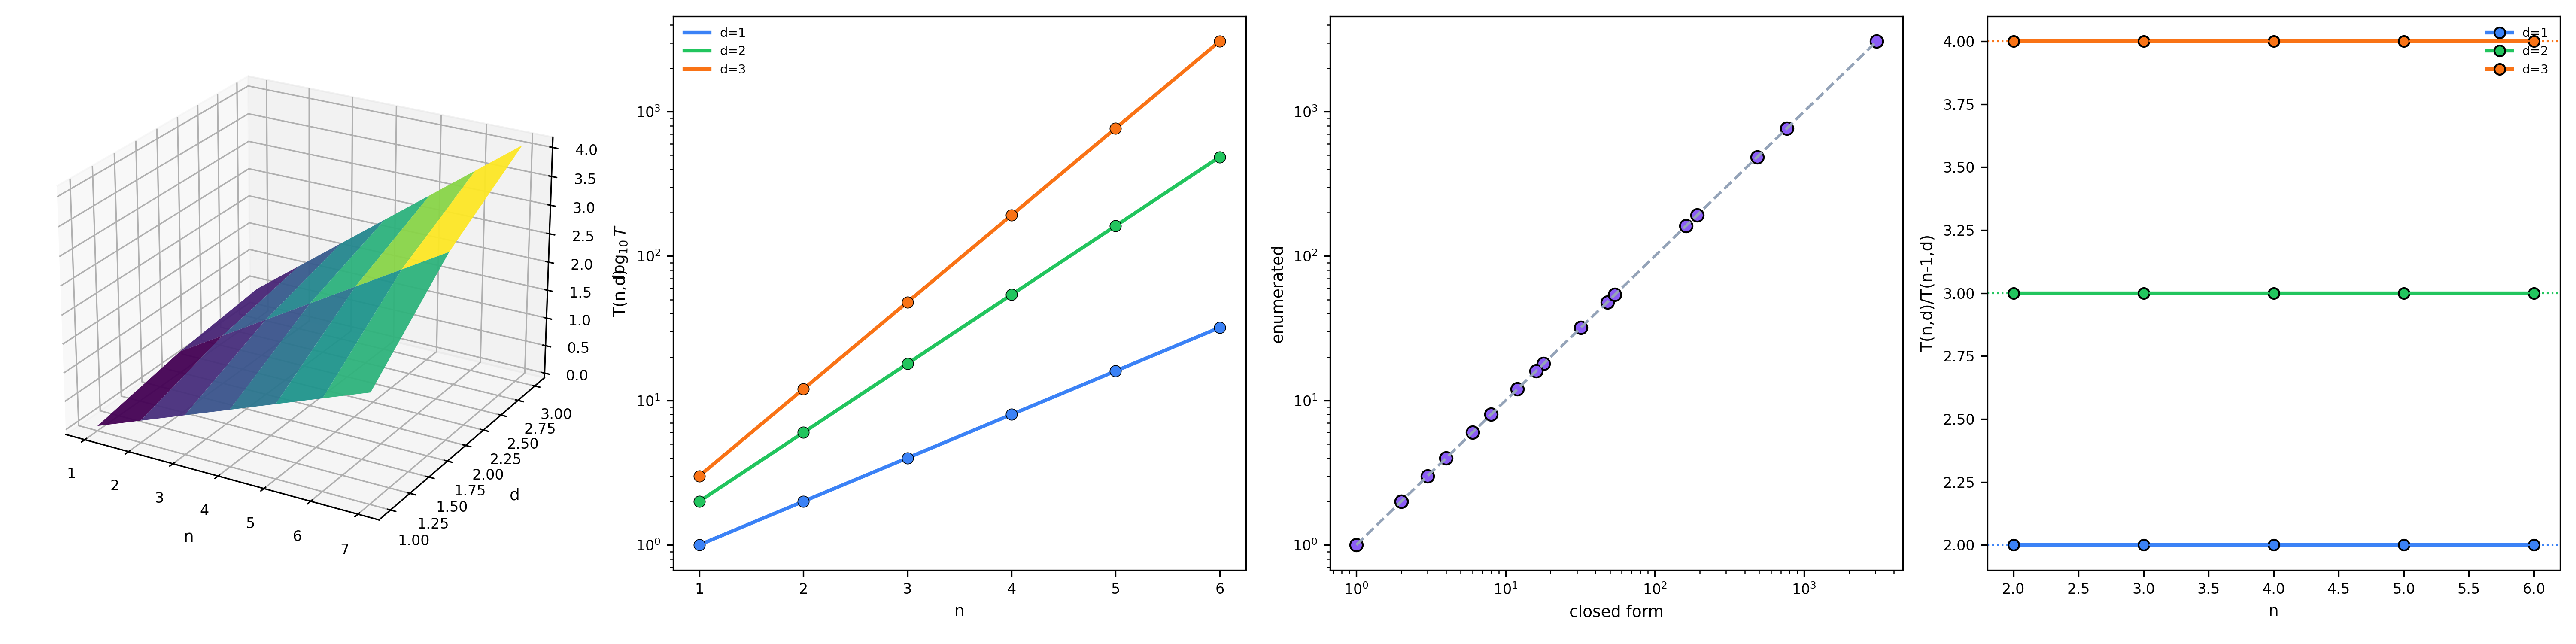
\includegraphics[width=\textwidth]{figures/panel_5_inflation.png}
    \caption{\textbf{Composition Inflation $T(n,d)=d(d+1)^{n-1}$.}
    (\textbf{A})~Three-dimensional surface of $\log_{10}T(n,d)$ over trajectory length $n$ and direction count $d$ (viridis); the surface rises steeply in $n$ and steepens with $d$, the exponential proliferation of distinguishable propagation trajectories with depth.
    (\textbf{B})~Trajectory count $T(n,d)$ on a logarithmic $y$-axis versus $n$ for $d=1,2,3$ (coloured lines), with directly enumerated counts (points) lying on the closed-form curves; enumeration and closed form agree exactly for every case computed.
    (\textbf{C})~Enumerated count versus closed form $d(d+1)^{n-1}$ on log--log axes; all points lie on the identity diagonal (grey dashed), the exact match of the brute-force enumeration to the formula.
    (\textbf{D})~Growth ratio $T(n,d)/T(n-1,d)$ versus $n$ for $d=1,2,3$ (coloured lines), each flat at its predicted value $d+1$ (dotted guides): the per-step branching factor is exactly $d+1$ (the $d$ moves plus the stay-option).}
    \label{fig:panel_inflation}
\end{figure*}

% ---------------------------------------------------------------------
\begin{figure*}[!htbp]
    \centering
    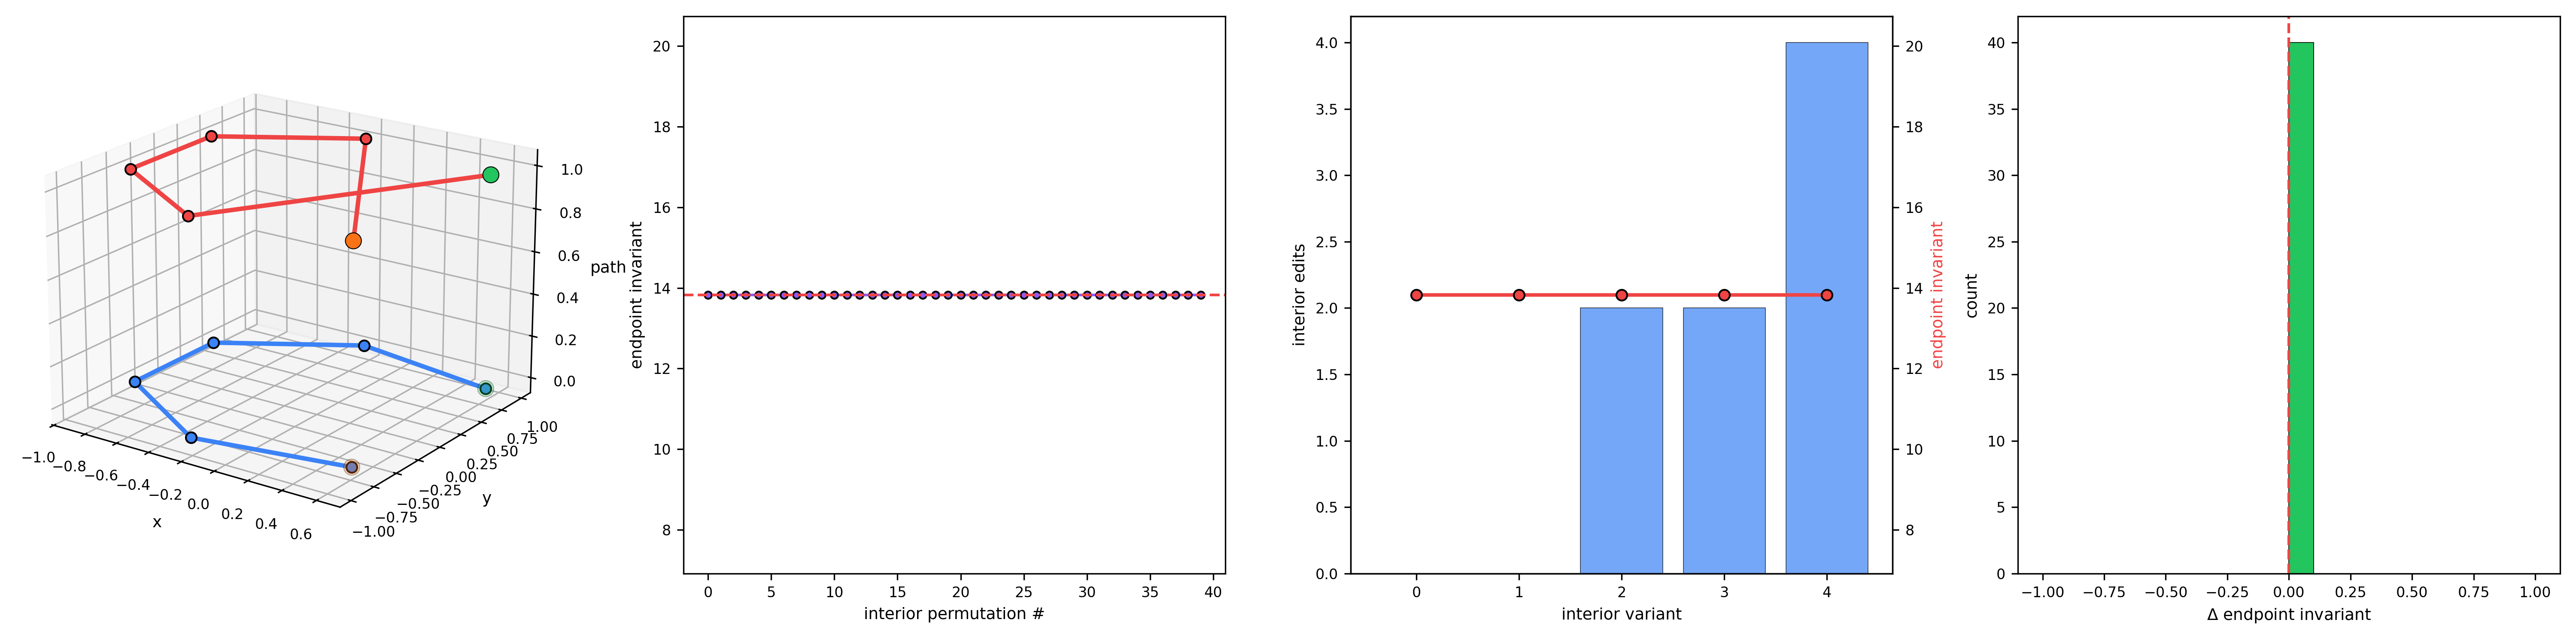
\includegraphics[width=\textwidth]{figures/panel_6_opacity.png}
    \caption{\textbf{Path Opacity: the Interior is Free.}
    (\textbf{A})~Three-dimensional rendering of two propagations sharing the same input (green) and output (orange) but distinct interior vertex orders, drawn on a circular item layout and lifted onto two path-index planes (blue and red). The two interiors differ while the endpoints coincide.
    (\textbf{B})~The endpoint invariant (the output's minimum-cut cost against the medium) across $40$ interior permutations; it is constant (points on the red dashed level), because the invariant depends only on the endpoints (Theorem~\ref{thm:path-opacity}).
    (\textbf{C})~Interior edit distance from a reference path (blue bars, left axis) growing across interior variants, against the endpoint invariant (red line, right axis) which stays flat: the interior may be edited arbitrarily without moving the endpoint invariant.
    (\textbf{D})~Distribution of the change $\Delta$ in the endpoint invariant across interior variants, a single spike at zero (red dashed): no interior rearrangement changes the endpoint invariant, so same-endpoint propagations are indistinguishable.}
    \label{fig:panel_opacity}
\end{figure*}

% ---------------------------------------------------------------------
\begin{figure*}[!htbp]
    \centering
    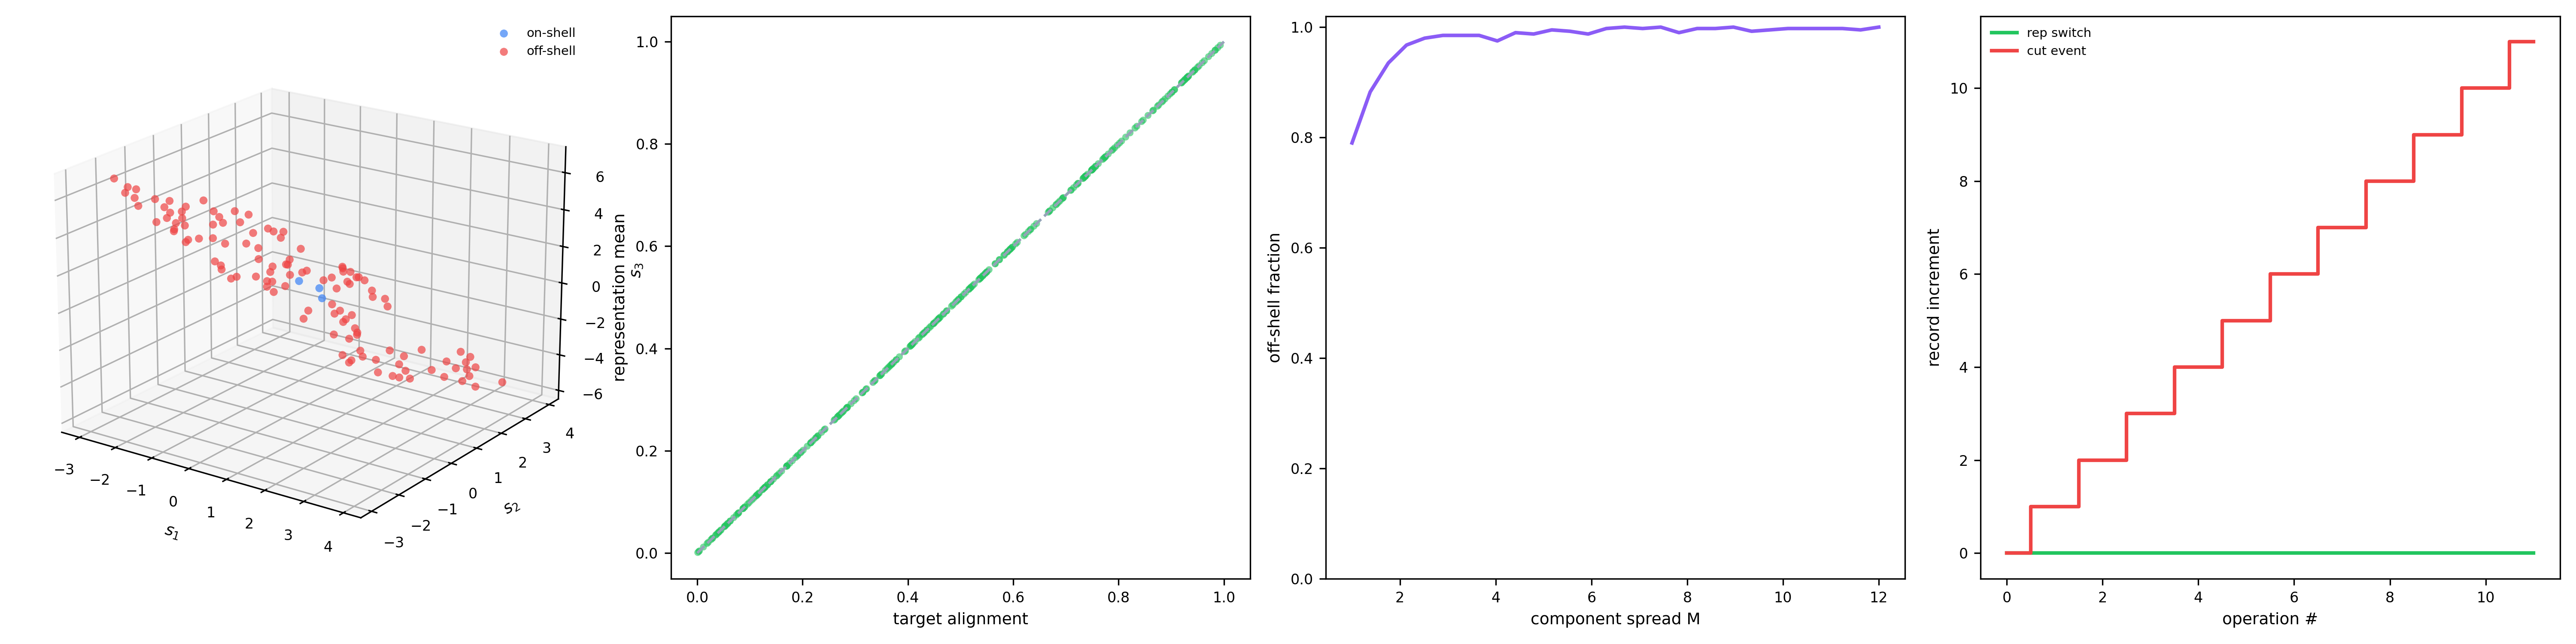
\includegraphics[width=\textwidth]{figures/panel_7_representation.png}
    \caption{\textbf{Representation Mobility and Mean Recovery.}
    (\textbf{A})~Three-dimensional scatter of $120$ three-component representations of a single item (alignment $0.5$) in $(s_1,s_2,s_3)$ space, coloured on-shell (blue, all components in $[0,1]$) or off-shell (red, some component outside): all lie on the mean-recovery plane $\tfrac13\sum s_j=0.5$, with off-shell components fully admissible (Theorem~\ref{thm:rep-mobility}).
    (\textbf{B})~Representation mean versus target alignment over $300$ random fibres and targets; every point lies on the diagonal (grey dashed): the component mean recovers the target exactly, whatever the individual components.
    (\textbf{C})~Off-shell fraction versus the component spread $M$; as the admissible spread grows the fraction of representations with an out-of-range component rises toward one, the freedom of the fibre to pass through ``impossible'' components while keeping the physical mean.
    (\textbf{D})~Record increment per operation: a representation switch (green) adds nothing to the committed record, while a cut event (red) increments it---switching representation commits no cut and leaves admissibility unchanged (Corollary~\ref{cor:mobility-required}).}
    \label{fig:panel_representation}
\end{figure*}

% ---------------------------------------------------------------------
\begin{figure*}[!htbp]
    \centering
    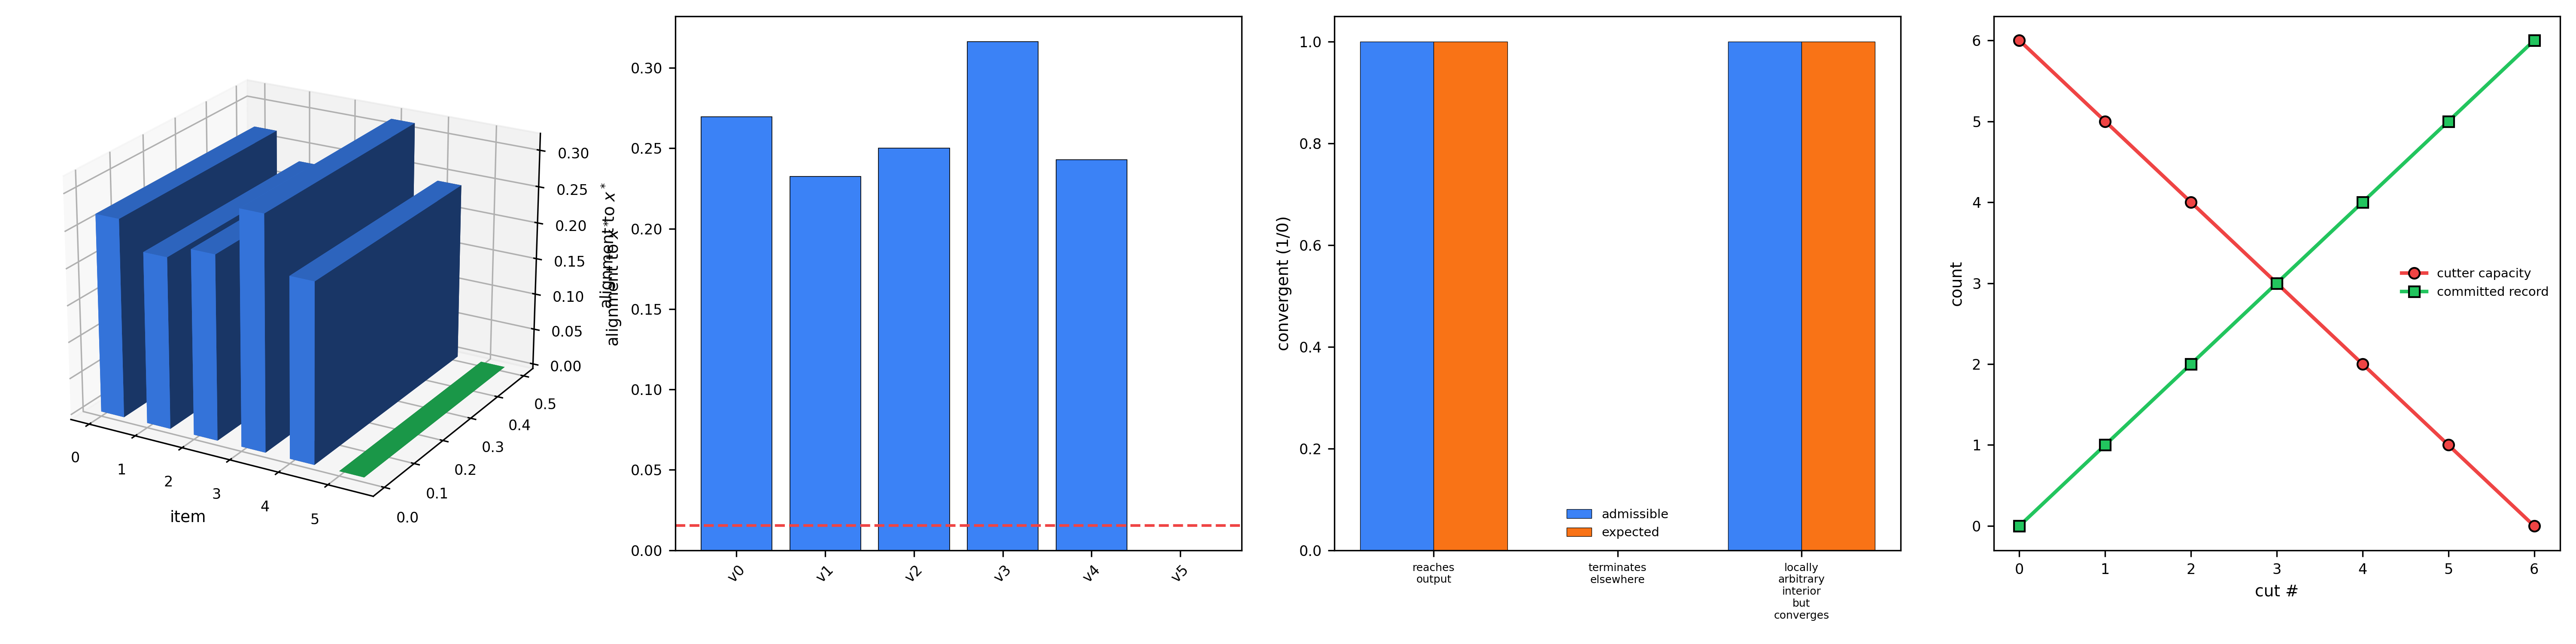
\includegraphics[width=\textwidth]{figures/panel_8_convergence_cut.png}
    \caption{\textbf{Convergence Admissibility and the One-Use Cut.}
    (\textbf{A})~Three-dimensional bar chart of each item's alignment to the output $x^{*}$ (cut cost to $x^{*}$ over total weight), the output bar green and the rest blue; only the output sits at the floor, the terminal accountable state of an admissible propagation.
    (\textbf{B})~Alignment to $x^{*}$ per item with the floor alignment $\beta/\Omega$ marked (red dashed); the output (green) alone reaches the floor, so a propagation is admissible exactly when it terminates there (Theorem~\ref{thm:admissibility}).
    (\textbf{C})~Convergence outcome for three cases---reaching the output, terminating elsewhere, and a locally arbitrary interior that nonetheless converges---with admissible (blue) and expected (orange) bars coinciding in each: admissibility tracks convergence to the output and nothing else, local steps being free.
    (\textbf{D})~The one-use, self-blunting cut: the cutter's uncommitted capacity (red) decreases by one per cut while the committed record (green) increases by one, the two crossing as capacity is spent. A cut commits once and blunts the cutter; the perfect repeatable traceless cut ($\beta=0$, record unchanged) cannot occur (Theorem~\ref{thm:one-use}, Theorem~\ref{thm:blunt}, Theorem~\ref{thm:no-perfect}).}
    \label{fig:panel_convergence_cut}
\end{figure*}
 or copy individually.
% =====================================================================

% ---------------------------------------------------------------------
\begin{figure*}[!htbp]
    \centering
    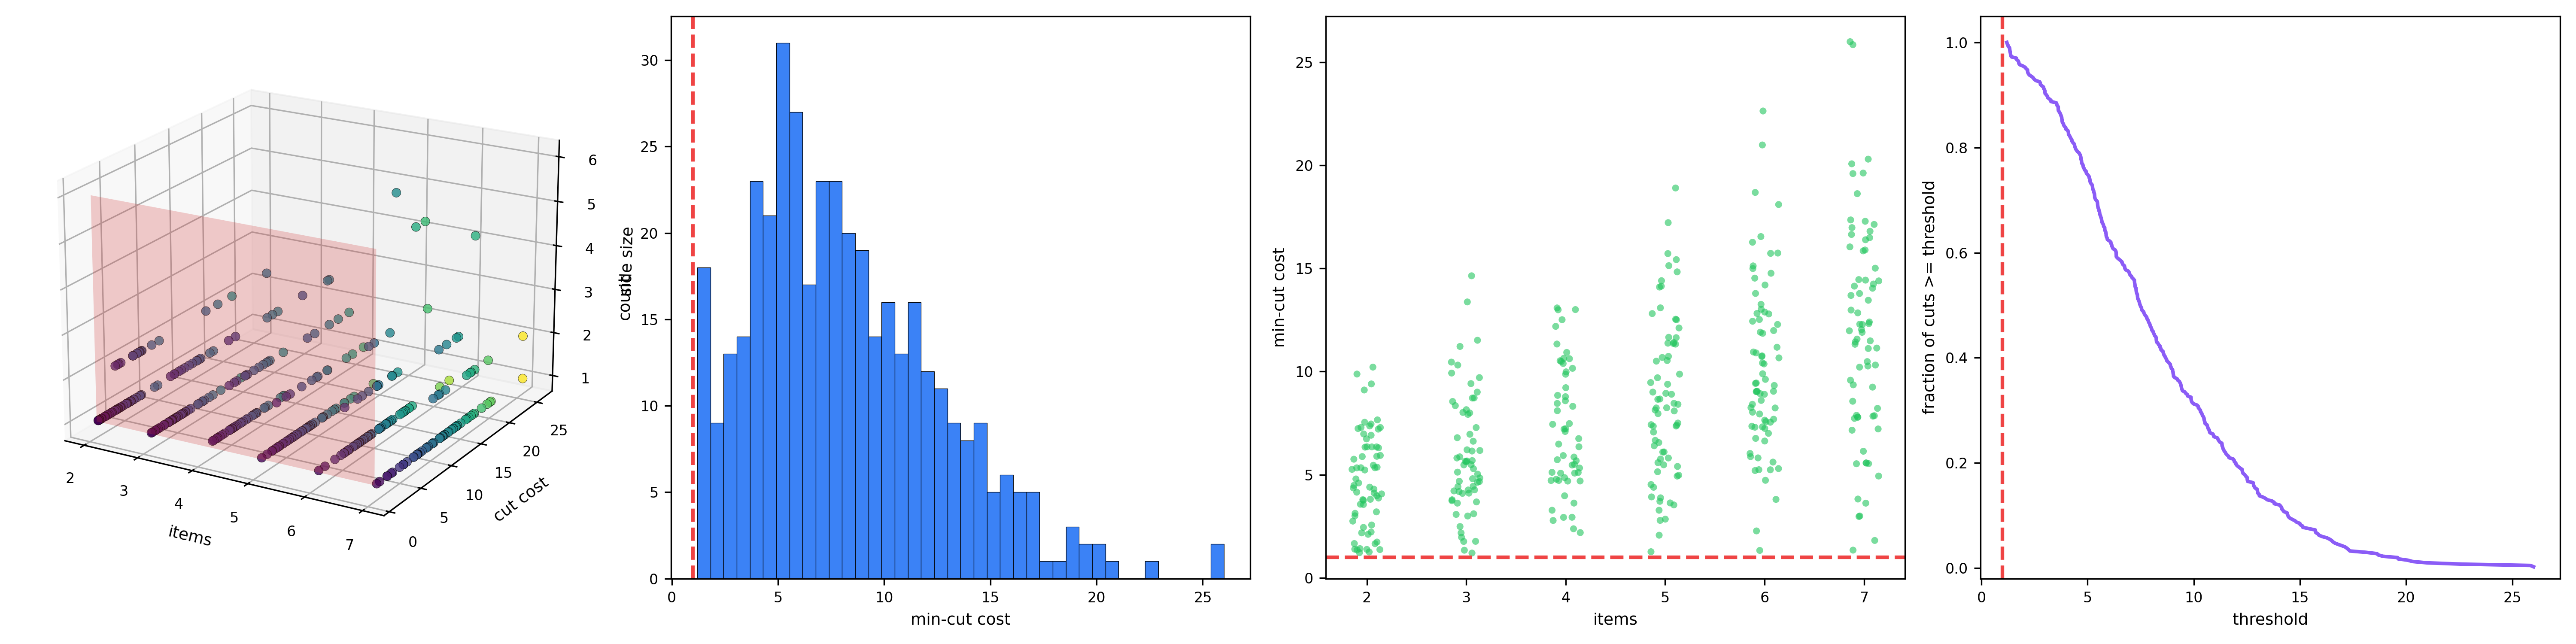
\includegraphics[width=\textwidth]{figures/panel_1_floor.png}
    \caption{\textbf{The Floor: Minimum Cuts over Random Contact Graphs.}
    (\textbf{A})~Three-dimensional scatter of $400$ random contact graphs in (number of items, minimum-cut cost, cut-side size) space, points coloured by cut cost (viridis), with the floor plane at cost $\beta$ drawn in red. Every point lies on or above the floor plane: no item is separated from the medium for less than $\beta$ (Theorem~\ref{thm:floor}).
    (\textbf{B})~Distribution of the exact minimum-cut costs (\texttt{networkx} max-flow) across the $400$ graphs, with the floor $\beta$ marked (red dashed). No mass falls below $\beta$, the absence of any sharp cut (Corollary~\ref{cor:no-sharp}).
    (\textbf{C})~Minimum-cut cost versus number of items (jittered) for all graphs; the entire cloud sits above the floor line $\beta$ (red dashed) independently of graph order, confirming the bound holds at every size.
    (\textbf{D})~Survival curve: the fraction of cuts with cost at least a given threshold, dropping from one only after the threshold passes $\beta$ (red dashed). The fraction at or above $\beta$ is unity---every one of the $300$ validated cuts clears the floor.}
    \label{fig:panel_floor}
\end{figure*}

% ---------------------------------------------------------------------
\begin{figure*}[!htbp]
    \centering
    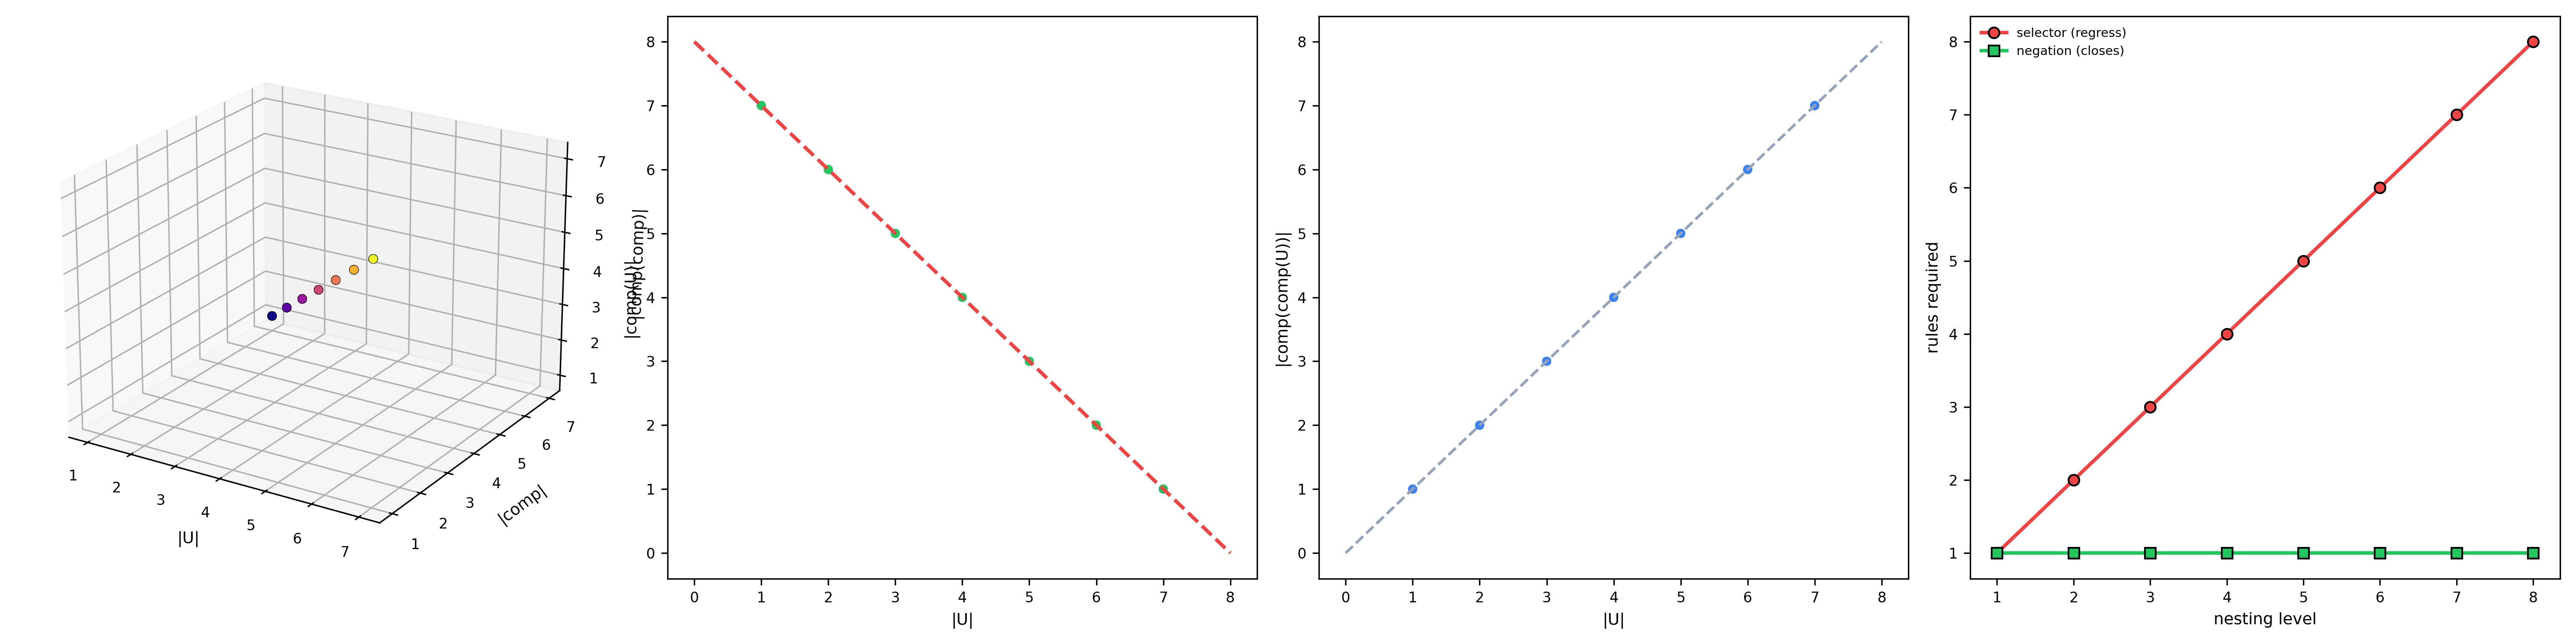
\includegraphics[width=\textwidth]{figures/panel_2_negation.png}
    \caption{\textbf{Individuation by Negation: the Complement Involution.}
    (\textbf{A})~Three-dimensional scatter of $200$ random subsets of an eight-element whole in $(|U|,\,|\co U|,\,|\co\co U|)$ space, coloured by $|U|$ (plasma). Every point satisfies $|\co\co U|=|U|$: double complementation returns the part, the involution underlying Theorem~\ref{thm:negation}.
    (\textbf{B})~Subset size $|U|$ versus complement size $|\co U|$; all points lie on the conservation line $|U|+|\co U|=8$ (red dashed): the complement is exactly ``the rest,'' fixed once the whole is given.
    (\textbf{C})~Double-complement size $|\co\co U|$ versus $|U|$ on the identity diagonal (grey dashed); the points coincide with the diagonal, so $\co$ is its own inverse and $\co U$ determines $U$ uniquely.
    (\textbf{D})~Rules required to fix a part as a function of nesting level: a positive (selector-based) rule regresses without bound (red), while negation closes at level one (green). The diverging red curve is the selector regress that Theorem~\ref{thm:negation} excludes; the flat green line is complementation, which needs only the whole.}
    \label{fig:panel_negation}
\end{figure*}

% ---------------------------------------------------------------------
\begin{figure*}[!htbp]
    \centering
    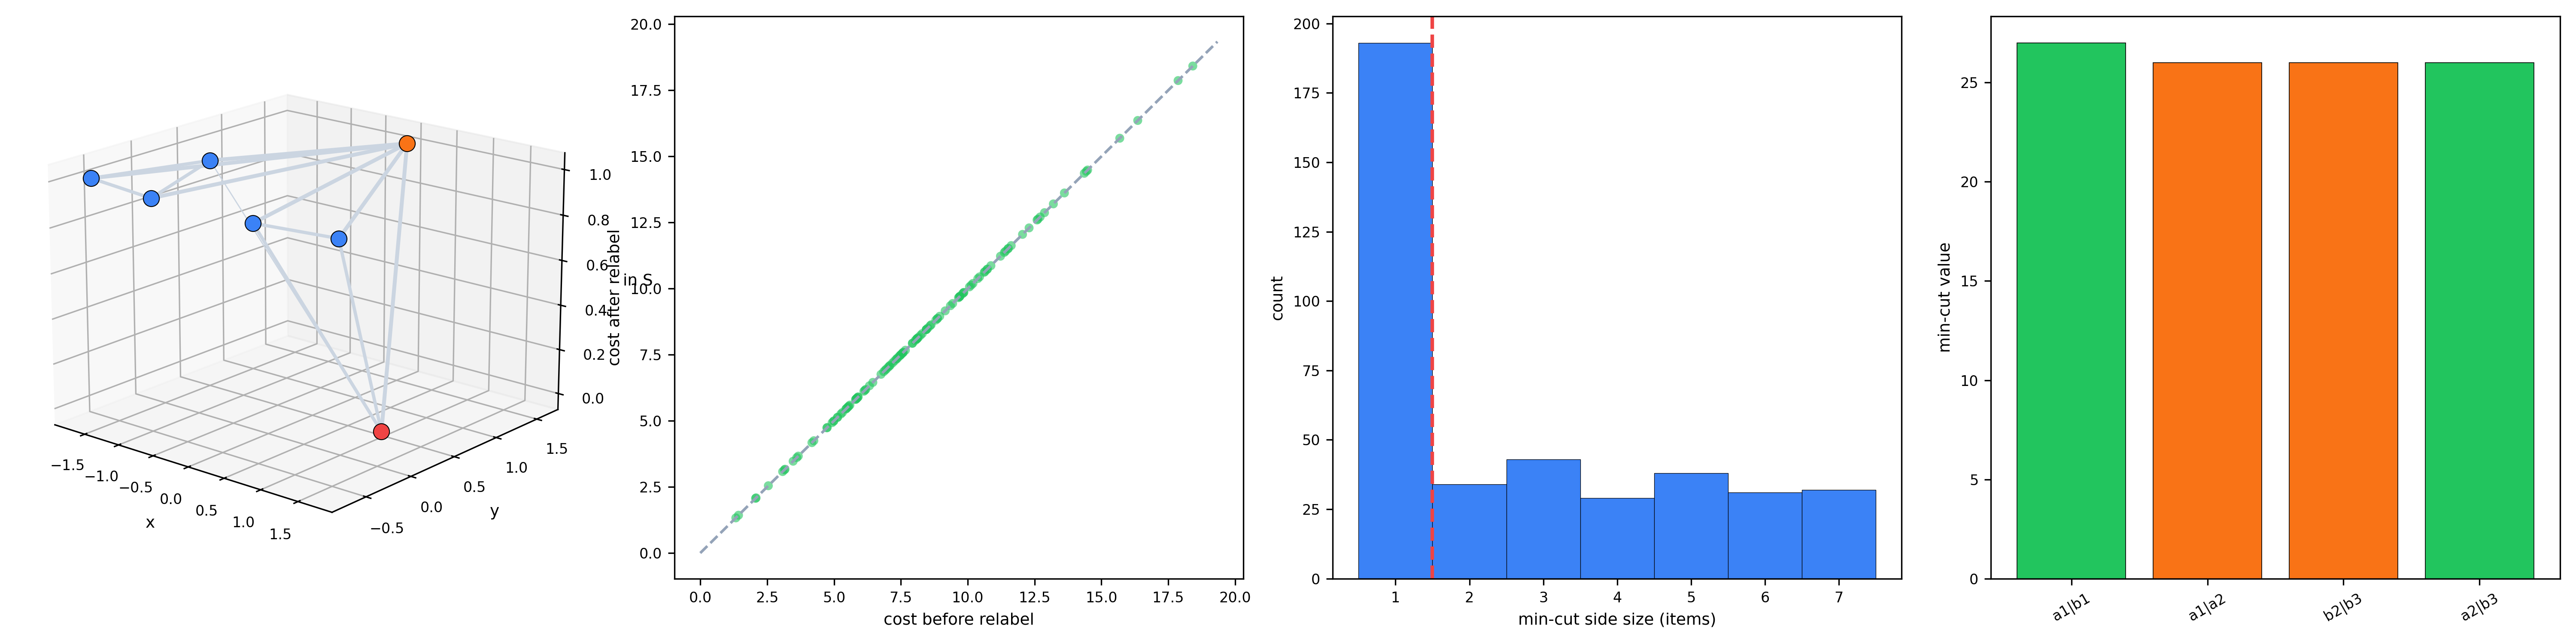
\includegraphics[width=\textwidth]{figures/panel_3_identity.png}
    \caption{\textbf{Identity as an Invariant Region, Never a Point.}
    (\textbf{A})~Three-dimensional rendering of the two-cluster contact graph: items (blue if on the source side $S$ of the minimum cut, red otherwise) and the medium (orange) at the origin, lifted on the vertical axis by cut membership, with edges drawn at width proportional to weight. The minimum cut places a multi-item set on the source side---identity is borne by a region, not a single vertex.
    (\textbf{B})~Minimum-cut cost before versus after a random relabelling (weighted isomorphism) of the items, over $120$ graphs; all points lie on the identity diagonal (grey dashed), so the cost is label-independent (Theorem~\ref{thm:invariant}).
    (\textbf{C})~Distribution of minimum-cut side sizes over $400$ random graphs; the mass lies predominantly above one item (the threshold at $1.5$, red dashed), the empirical content of ``the minimising side is in general not a singleton'' (Theorem~\ref{thm:region}).
    (\textbf{D})~Minimum-cut value for four different separated pairs in the two-cluster instance: the cluster-separating pairs (green) realise the cheap inter-cluster cut, while same-cluster pairs (orange) cost more, showing the cut value is a property of the partition, not of a chosen endpoint.}
    \label{fig:panel_identity}
\end{figure*}

% ---------------------------------------------------------------------
\begin{figure*}[!htbp]
    \centering
    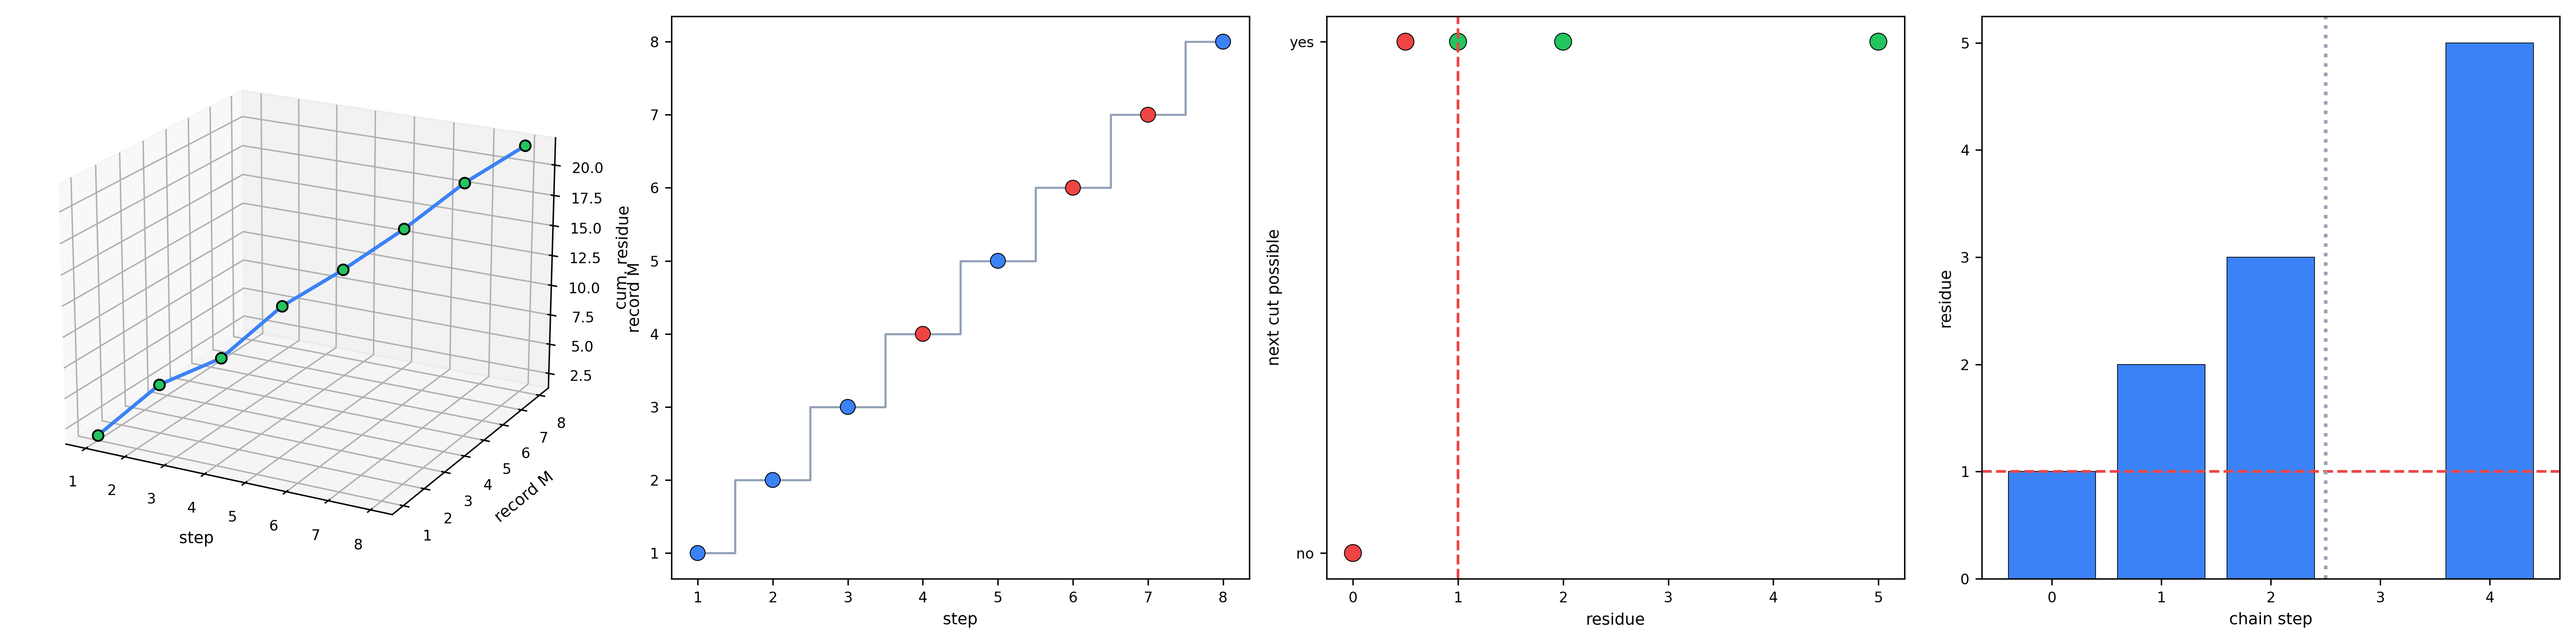
\includegraphics[width=\textwidth]{figures/panel_4_record_residue.png}
    \caption{\textbf{The Monotone Record and the Residue Propagator.}
    (\textbf{A})~Three-dimensional trajectory of a process in (step, committed record $M$, cumulative residue) space: the record climbs monotonically while the residue accumulates, the two coupled because each cut deposits a residue and increments the record (Theorem~\ref{thm:monotone}, Theorem~\ref{thm:propagator}).
    (\textbf{B})~Committed record $M$ versus step for an eight-event process; the staircase strictly increases, and the ``undo'' events (red points) increment the record exactly as forward cuts (blue) do---un-committing is itself a further cut, so the record never returns.
    (\textbf{C})~Whether a distinct next cut is possible (yes/no) versus the residue of the current cut; the transition occurs at residue zero, with points coloured green when the residue clears the floor $\beta$ (red dashed) and red otherwise. Residue $>0$ is necessary and sufficient for the next cut.
    (\textbf{D})~Residue at each step of a five-step chain, bars blue where the residue clears the floor and red where it would vanish; the dashed floor line $\beta$ and the halt marker (grey dotted) show the chain stopping exactly where a residue would fall below $\beta$---no residue, no next event.}
    \label{fig:panel_record_residue}
\end{figure*}

% ---------------------------------------------------------------------
\begin{figure*}[!htbp]
    \centering
    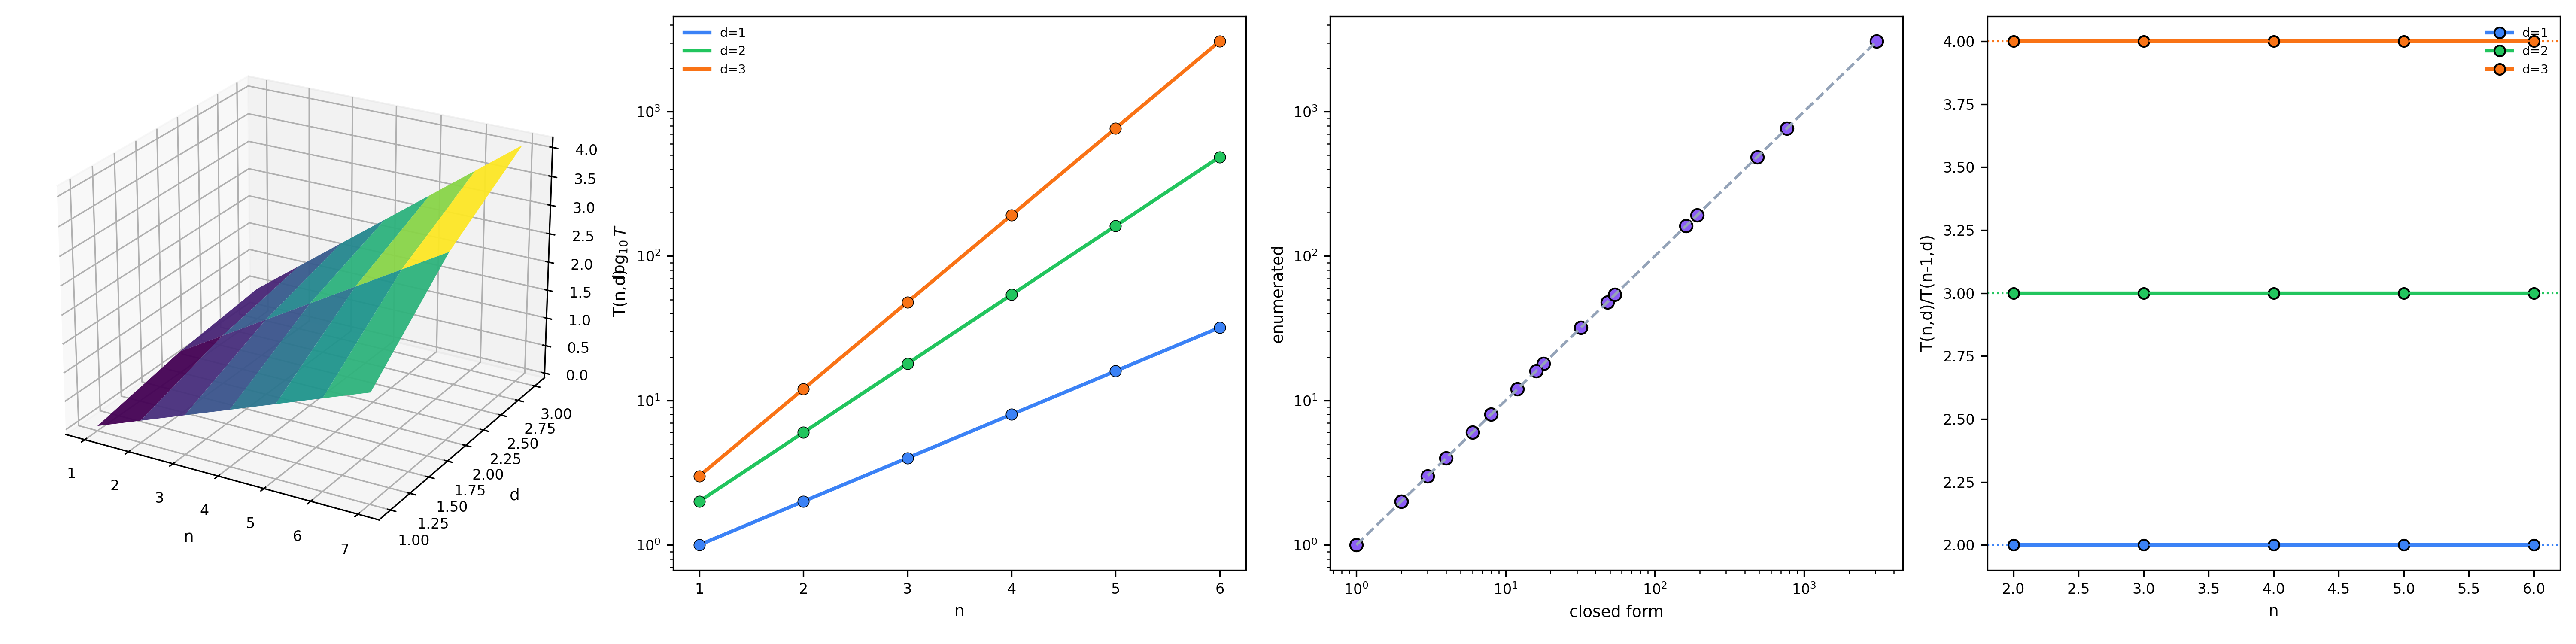
\includegraphics[width=\textwidth]{figures/panel_5_inflation.png}
    \caption{\textbf{Composition Inflation $T(n,d)=d(d+1)^{n-1}$.}
    (\textbf{A})~Three-dimensional surface of $\log_{10}T(n,d)$ over trajectory length $n$ and direction count $d$ (viridis); the surface rises steeply in $n$ and steepens with $d$, the exponential proliferation of distinguishable propagation trajectories with depth.
    (\textbf{B})~Trajectory count $T(n,d)$ on a logarithmic $y$-axis versus $n$ for $d=1,2,3$ (coloured lines), with directly enumerated counts (points) lying on the closed-form curves; enumeration and closed form agree exactly for every case computed.
    (\textbf{C})~Enumerated count versus closed form $d(d+1)^{n-1}$ on log--log axes; all points lie on the identity diagonal (grey dashed), the exact match of the brute-force enumeration to the formula.
    (\textbf{D})~Growth ratio $T(n,d)/T(n-1,d)$ versus $n$ for $d=1,2,3$ (coloured lines), each flat at its predicted value $d+1$ (dotted guides): the per-step branching factor is exactly $d+1$ (the $d$ moves plus the stay-option).}
    \label{fig:panel_inflation}
\end{figure*}

% ---------------------------------------------------------------------
\begin{figure*}[!htbp]
    \centering
    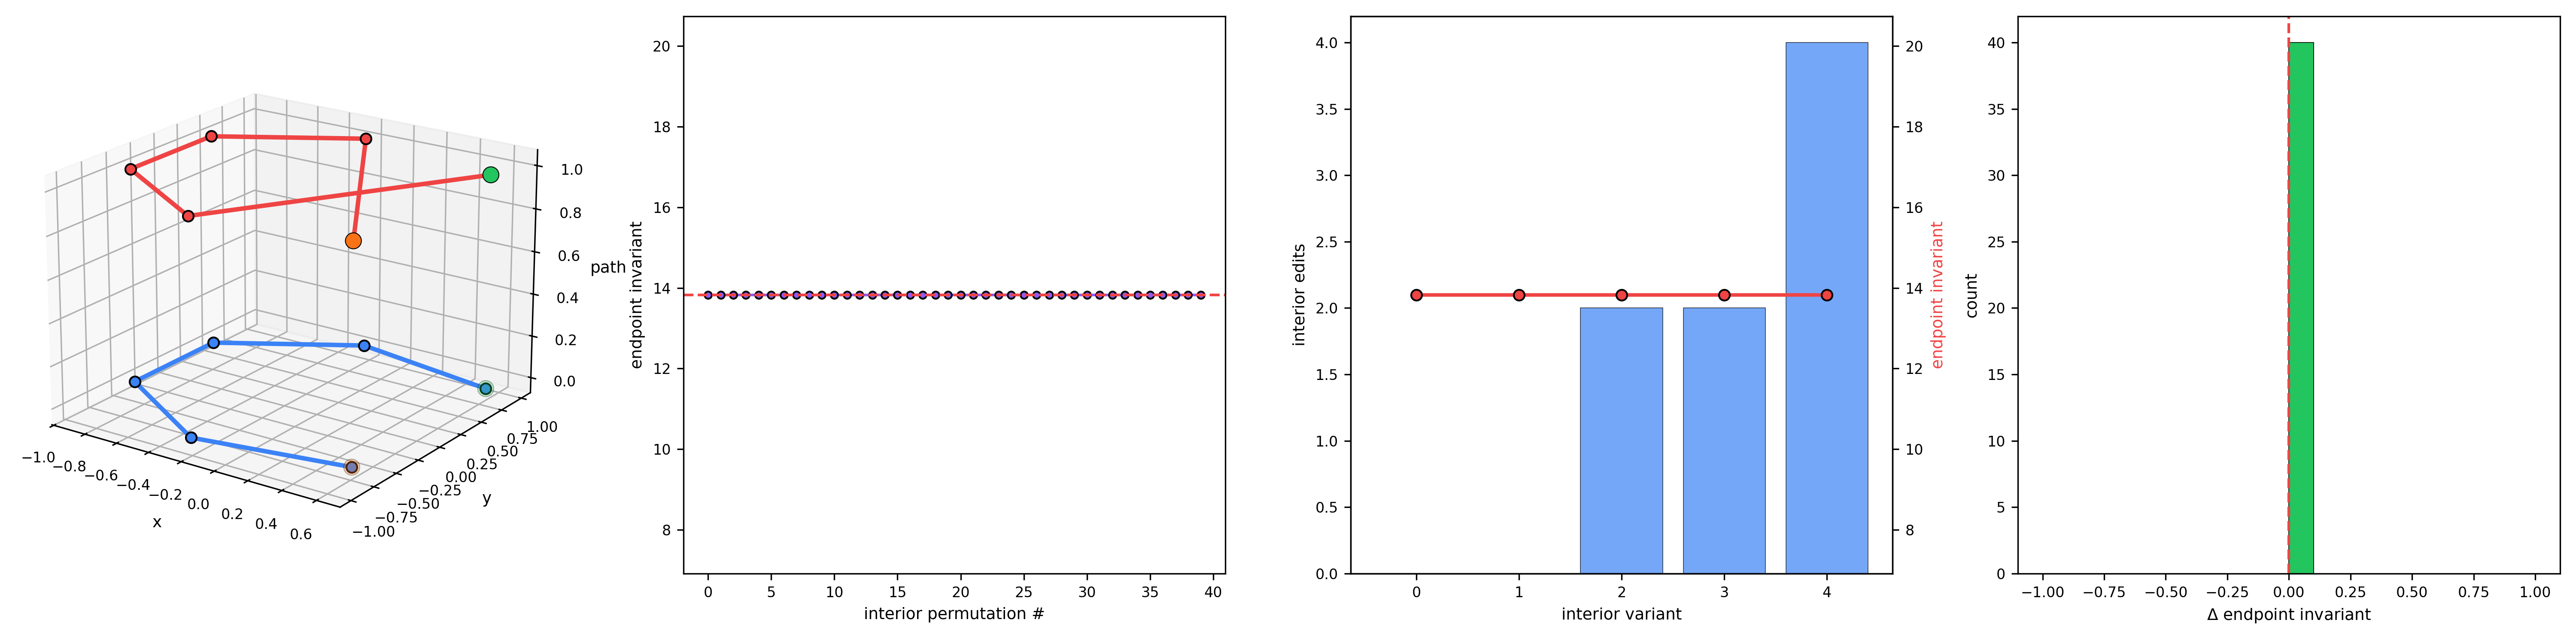
\includegraphics[width=\textwidth]{figures/panel_6_opacity.png}
    \caption{\textbf{Path Opacity: the Interior is Free.}
    (\textbf{A})~Three-dimensional rendering of two propagations sharing the same input (green) and output (orange) but distinct interior vertex orders, drawn on a circular item layout and lifted onto two path-index planes (blue and red). The two interiors differ while the endpoints coincide.
    (\textbf{B})~The endpoint invariant (the output's minimum-cut cost against the medium) across $40$ interior permutations; it is constant (points on the red dashed level), because the invariant depends only on the endpoints (Theorem~\ref{thm:path-opacity}).
    (\textbf{C})~Interior edit distance from a reference path (blue bars, left axis) growing across interior variants, against the endpoint invariant (red line, right axis) which stays flat: the interior may be edited arbitrarily without moving the endpoint invariant.
    (\textbf{D})~Distribution of the change $\Delta$ in the endpoint invariant across interior variants, a single spike at zero (red dashed): no interior rearrangement changes the endpoint invariant, so same-endpoint propagations are indistinguishable.}
    \label{fig:panel_opacity}
\end{figure*}

% ---------------------------------------------------------------------
\begin{figure*}[!htbp]
    \centering
    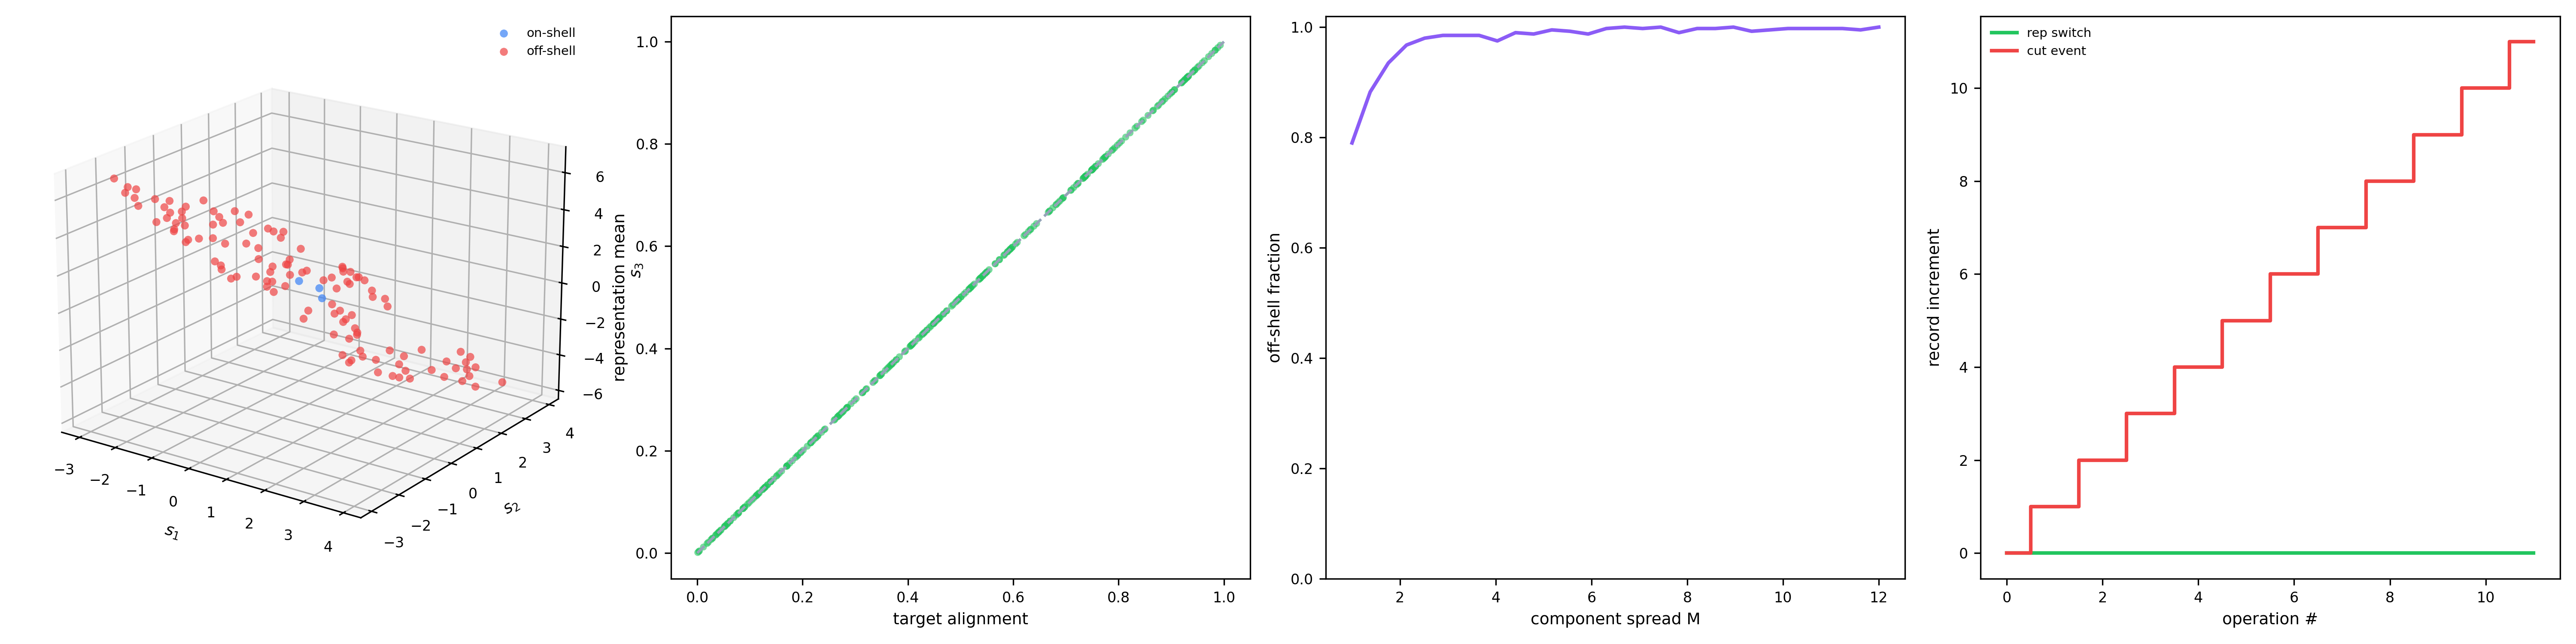
\includegraphics[width=\textwidth]{figures/panel_7_representation.png}
    \caption{\textbf{Representation Mobility and Mean Recovery.}
    (\textbf{A})~Three-dimensional scatter of $120$ three-component representations of a single item (alignment $0.5$) in $(s_1,s_2,s_3)$ space, coloured on-shell (blue, all components in $[0,1]$) or off-shell (red, some component outside): all lie on the mean-recovery plane $\tfrac13\sum s_j=0.5$, with off-shell components fully admissible (Theorem~\ref{thm:rep-mobility}).
    (\textbf{B})~Representation mean versus target alignment over $300$ random fibres and targets; every point lies on the diagonal (grey dashed): the component mean recovers the target exactly, whatever the individual components.
    (\textbf{C})~Off-shell fraction versus the component spread $M$; as the admissible spread grows the fraction of representations with an out-of-range component rises toward one, the freedom of the fibre to pass through ``impossible'' components while keeping the physical mean.
    (\textbf{D})~Record increment per operation: a representation switch (green) adds nothing to the committed record, while a cut event (red) increments it---switching representation commits no cut and leaves admissibility unchanged (Corollary~\ref{cor:mobility-required}).}
    \label{fig:panel_representation}
\end{figure*}

% ---------------------------------------------------------------------
\begin{figure*}[!htbp]
    \centering
    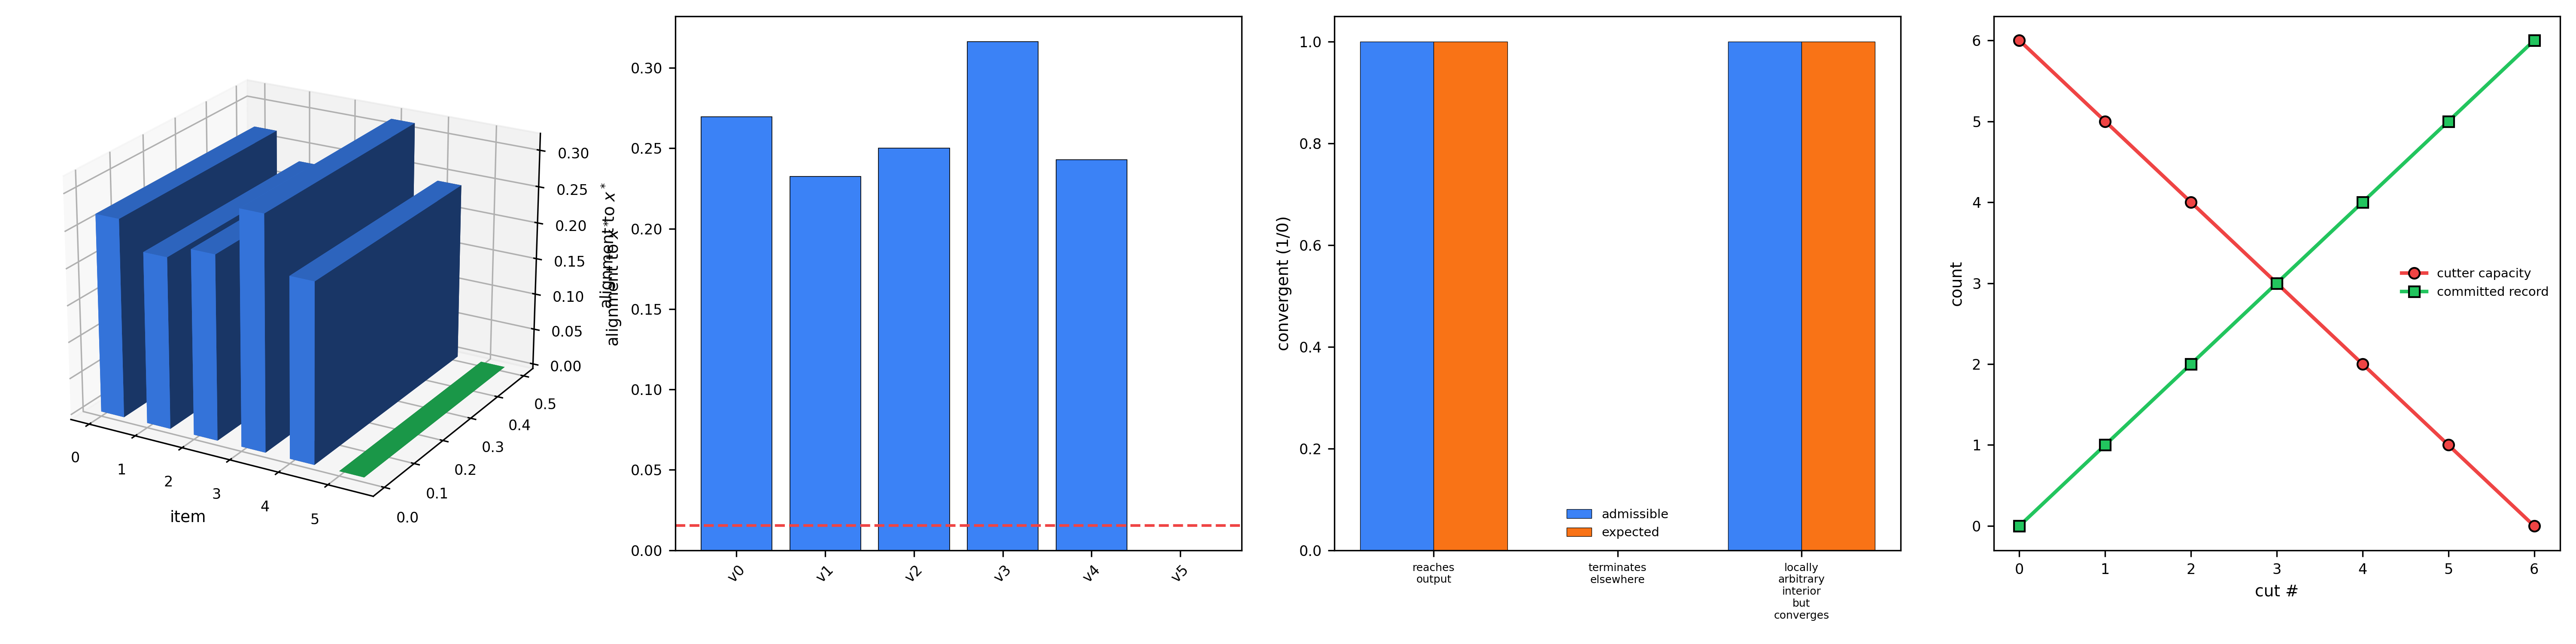
\includegraphics[width=\textwidth]{figures/panel_8_convergence_cut.png}
    \caption{\textbf{Convergence Admissibility and the One-Use Cut.}
    (\textbf{A})~Three-dimensional bar chart of each item's alignment to the output $x^{*}$ (cut cost to $x^{*}$ over total weight), the output bar green and the rest blue; only the output sits at the floor, the terminal accountable state of an admissible propagation.
    (\textbf{B})~Alignment to $x^{*}$ per item with the floor alignment $\beta/\Omega$ marked (red dashed); the output (green) alone reaches the floor, so a propagation is admissible exactly when it terminates there (Theorem~\ref{thm:admissibility}).
    (\textbf{C})~Convergence outcome for three cases---reaching the output, terminating elsewhere, and a locally arbitrary interior that nonetheless converges---with admissible (blue) and expected (orange) bars coinciding in each: admissibility tracks convergence to the output and nothing else, local steps being free.
    (\textbf{D})~The one-use, self-blunting cut: the cutter's uncommitted capacity (red) decreases by one per cut while the committed record (green) increases by one, the two crossing as capacity is spent. A cut commits once and blunts the cutter; the perfect repeatable traceless cut ($\beta=0$, record unchanged) cannot occur (Theorem~\ref{thm:one-use}, Theorem~\ref{thm:blunt}, Theorem~\ref{thm:no-perfect}).}
    \label{fig:panel_convergence_cut}
\end{figure*}
 or copy individually.
% =====================================================================

% ---------------------------------------------------------------------
\begin{figure*}[!htbp]
    \centering
    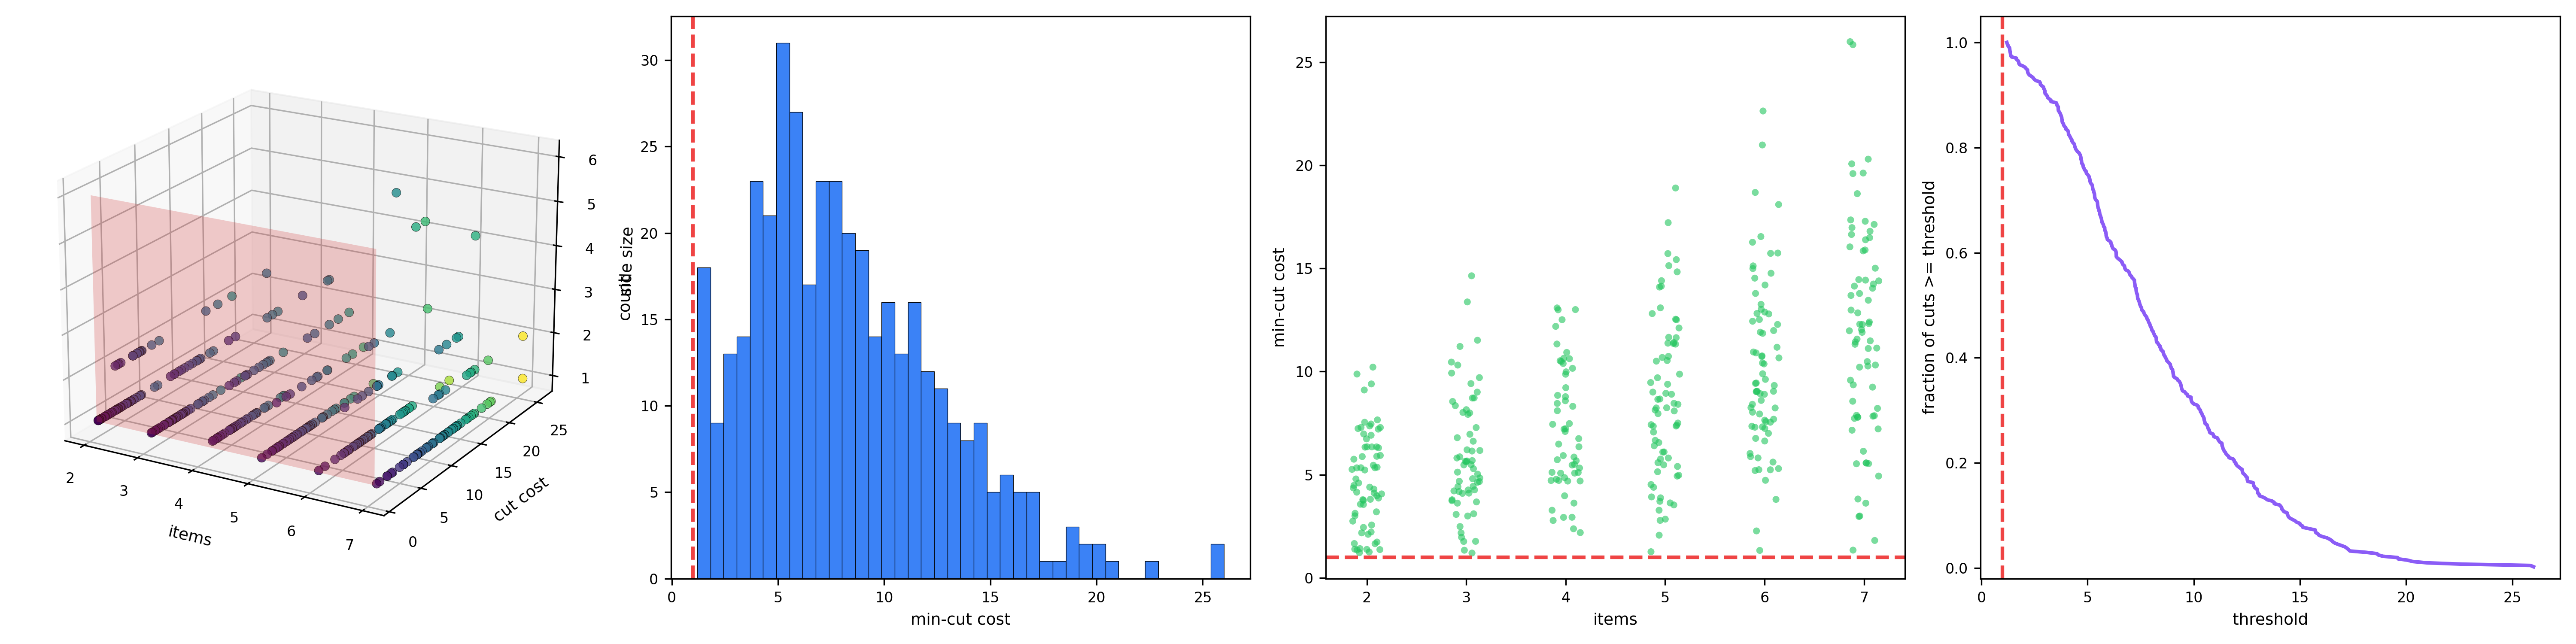
\includegraphics[width=\textwidth]{figures/panel_1_floor.png}
    \caption{\textbf{The Floor: Minimum Cuts over Random Contact Graphs.}
    (\textbf{A})~Three-dimensional scatter of $400$ random contact graphs in (number of items, minimum-cut cost, cut-side size) space, points coloured by cut cost (viridis), with the floor plane at cost $\beta$ drawn in red. Every point lies on or above the floor plane: no item is separated from the medium for less than $\beta$ (Theorem~\ref{thm:floor}).
    (\textbf{B})~Distribution of the exact minimum-cut costs (\texttt{networkx} max-flow) across the $400$ graphs, with the floor $\beta$ marked (red dashed). No mass falls below $\beta$, the absence of any sharp cut (Corollary~\ref{cor:no-sharp}).
    (\textbf{C})~Minimum-cut cost versus number of items (jittered) for all graphs; the entire cloud sits above the floor line $\beta$ (red dashed) independently of graph order, confirming the bound holds at every size.
    (\textbf{D})~Survival curve: the fraction of cuts with cost at least a given threshold, dropping from one only after the threshold passes $\beta$ (red dashed). The fraction at or above $\beta$ is unity---every one of the $300$ validated cuts clears the floor.}
    \label{fig:panel_floor}
\end{figure*}

% ---------------------------------------------------------------------
\begin{figure*}[!htbp]
    \centering
    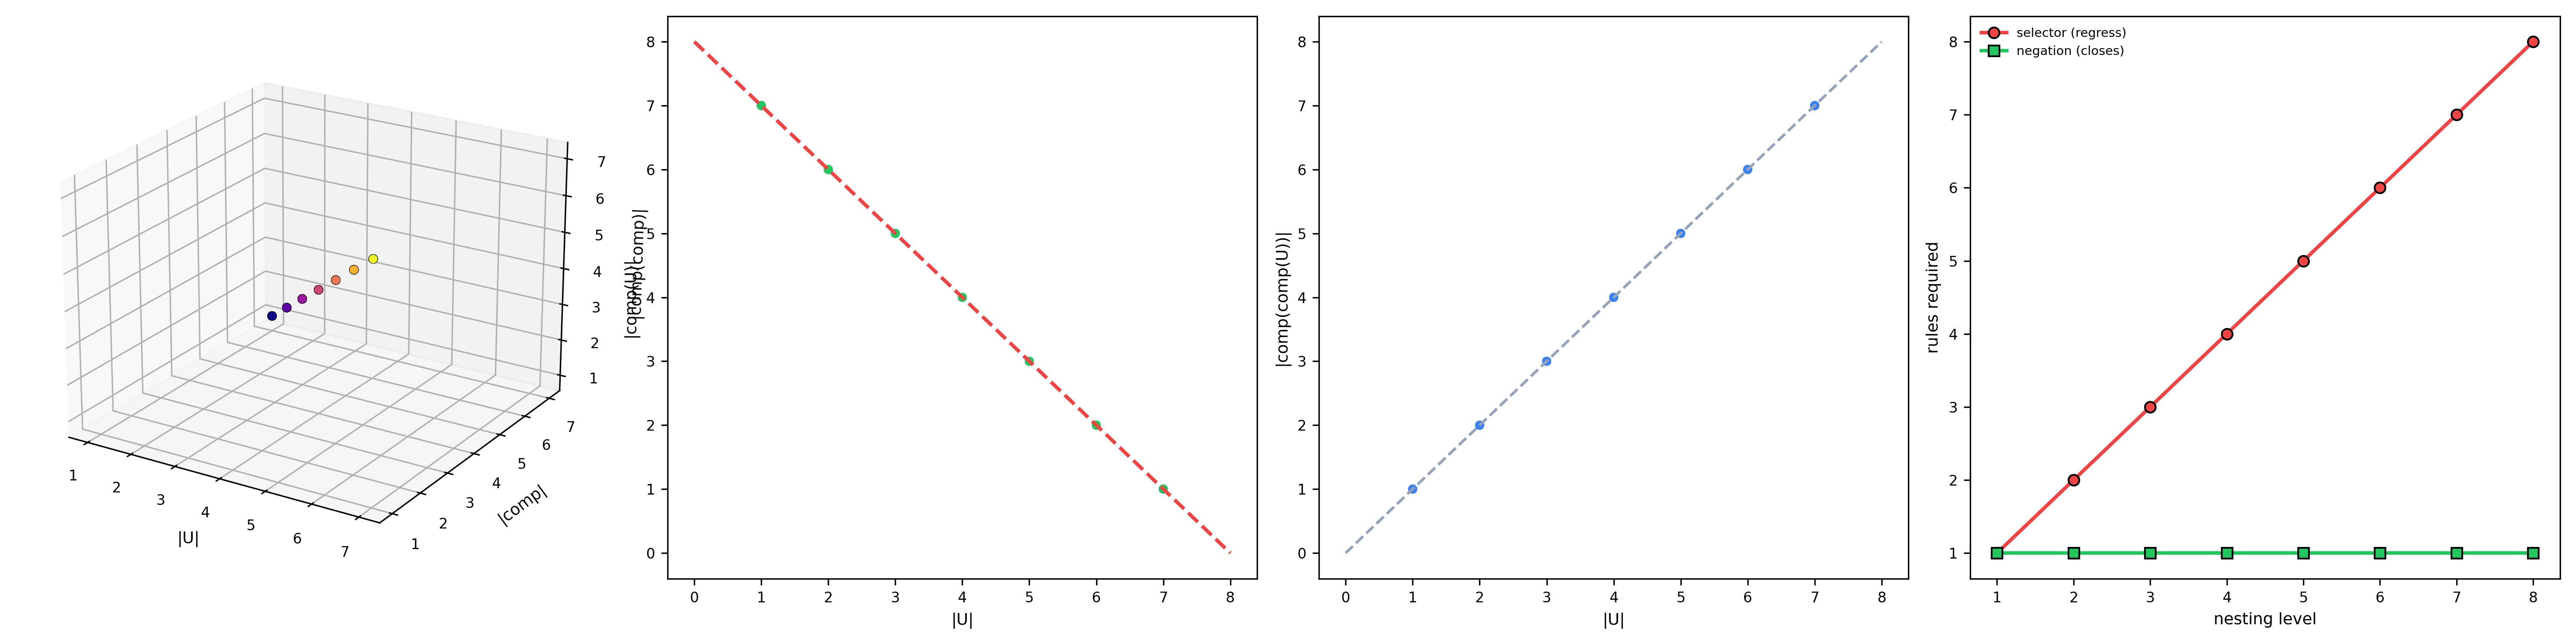
\includegraphics[width=\textwidth]{figures/panel_2_negation.png}
    \caption{\textbf{Individuation by Negation: the Complement Involution.}
    (\textbf{A})~Three-dimensional scatter of $200$ random subsets of an eight-element whole in $(|U|,\,|\co U|,\,|\co\co U|)$ space, coloured by $|U|$ (plasma). Every point satisfies $|\co\co U|=|U|$: double complementation returns the part, the involution underlying Theorem~\ref{thm:negation}.
    (\textbf{B})~Subset size $|U|$ versus complement size $|\co U|$; all points lie on the conservation line $|U|+|\co U|=8$ (red dashed): the complement is exactly ``the rest,'' fixed once the whole is given.
    (\textbf{C})~Double-complement size $|\co\co U|$ versus $|U|$ on the identity diagonal (grey dashed); the points coincide with the diagonal, so $\co$ is its own inverse and $\co U$ determines $U$ uniquely.
    (\textbf{D})~Rules required to fix a part as a function of nesting level: a positive (selector-based) rule regresses without bound (red), while negation closes at level one (green). The diverging red curve is the selector regress that Theorem~\ref{thm:negation} excludes; the flat green line is complementation, which needs only the whole.}
    \label{fig:panel_negation}
\end{figure*}

% ---------------------------------------------------------------------
\begin{figure*}[!htbp]
    \centering
    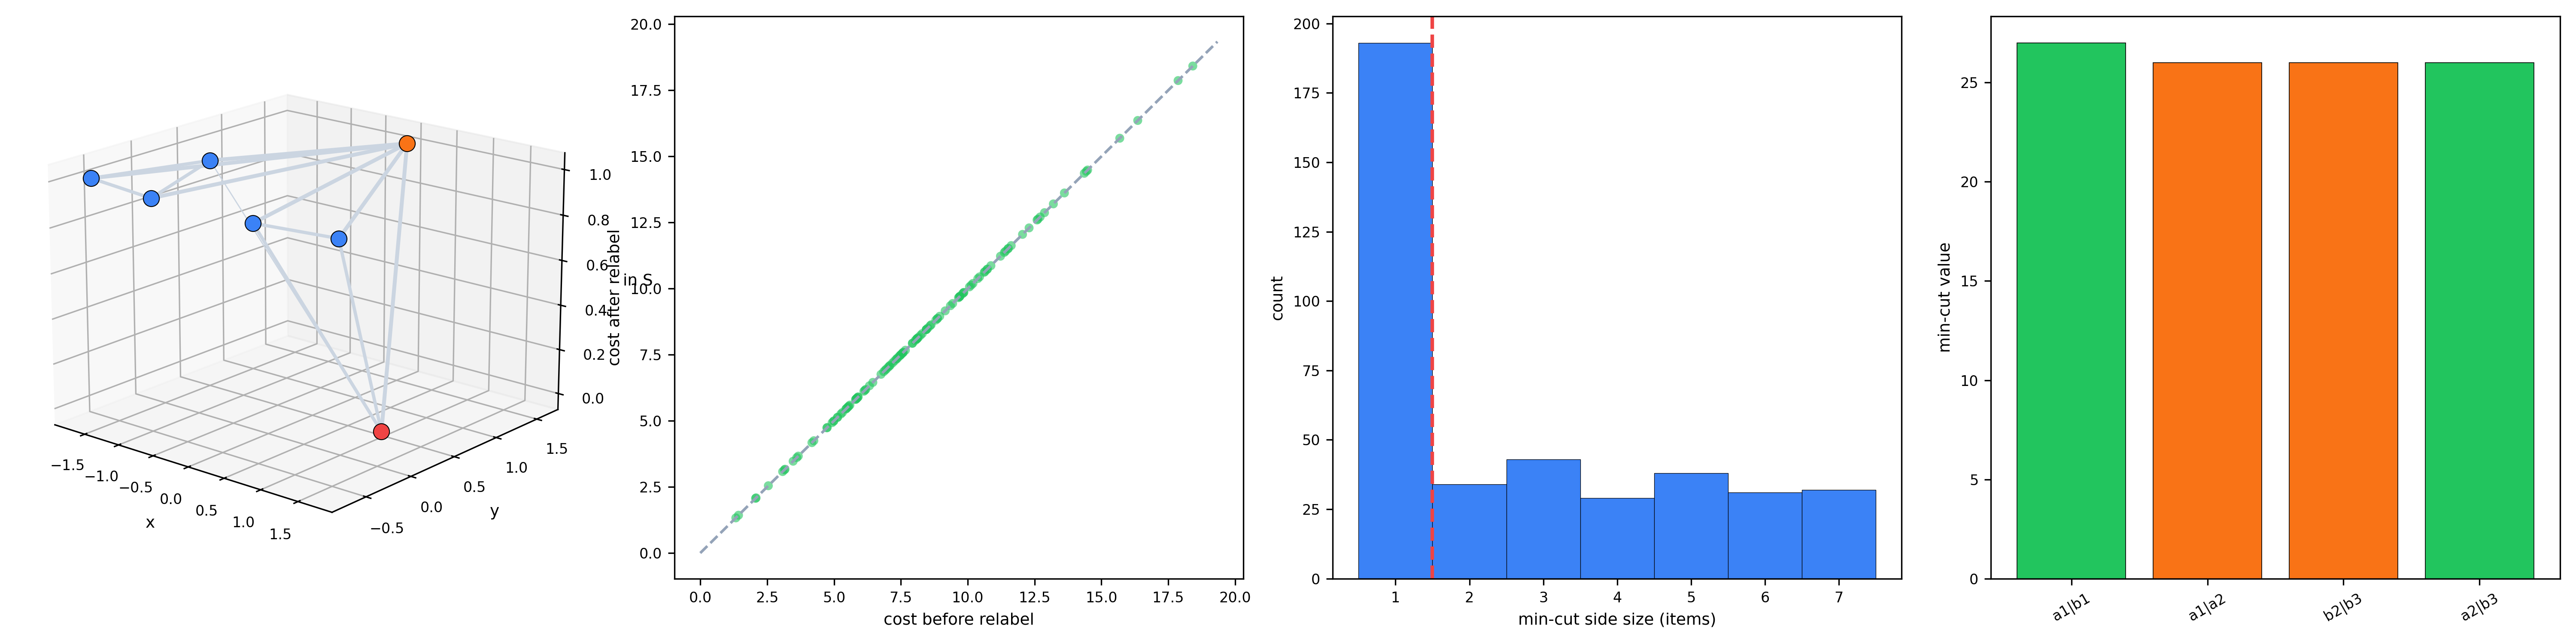
\includegraphics[width=\textwidth]{figures/panel_3_identity.png}
    \caption{\textbf{Identity as an Invariant Region, Never a Point.}
    (\textbf{A})~Three-dimensional rendering of the two-cluster contact graph: items (blue if on the source side $S$ of the minimum cut, red otherwise) and the medium (orange) at the origin, lifted on the vertical axis by cut membership, with edges drawn at width proportional to weight. The minimum cut places a multi-item set on the source side---identity is borne by a region, not a single vertex.
    (\textbf{B})~Minimum-cut cost before versus after a random relabelling (weighted isomorphism) of the items, over $120$ graphs; all points lie on the identity diagonal (grey dashed), so the cost is label-independent (Theorem~\ref{thm:invariant}).
    (\textbf{C})~Distribution of minimum-cut side sizes over $400$ random graphs; the mass lies predominantly above one item (the threshold at $1.5$, red dashed), the empirical content of ``the minimising side is in general not a singleton'' (Theorem~\ref{thm:region}).
    (\textbf{D})~Minimum-cut value for four different separated pairs in the two-cluster instance: the cluster-separating pairs (green) realise the cheap inter-cluster cut, while same-cluster pairs (orange) cost more, showing the cut value is a property of the partition, not of a chosen endpoint.}
    \label{fig:panel_identity}
\end{figure*}

% ---------------------------------------------------------------------
\begin{figure*}[!htbp]
    \centering
    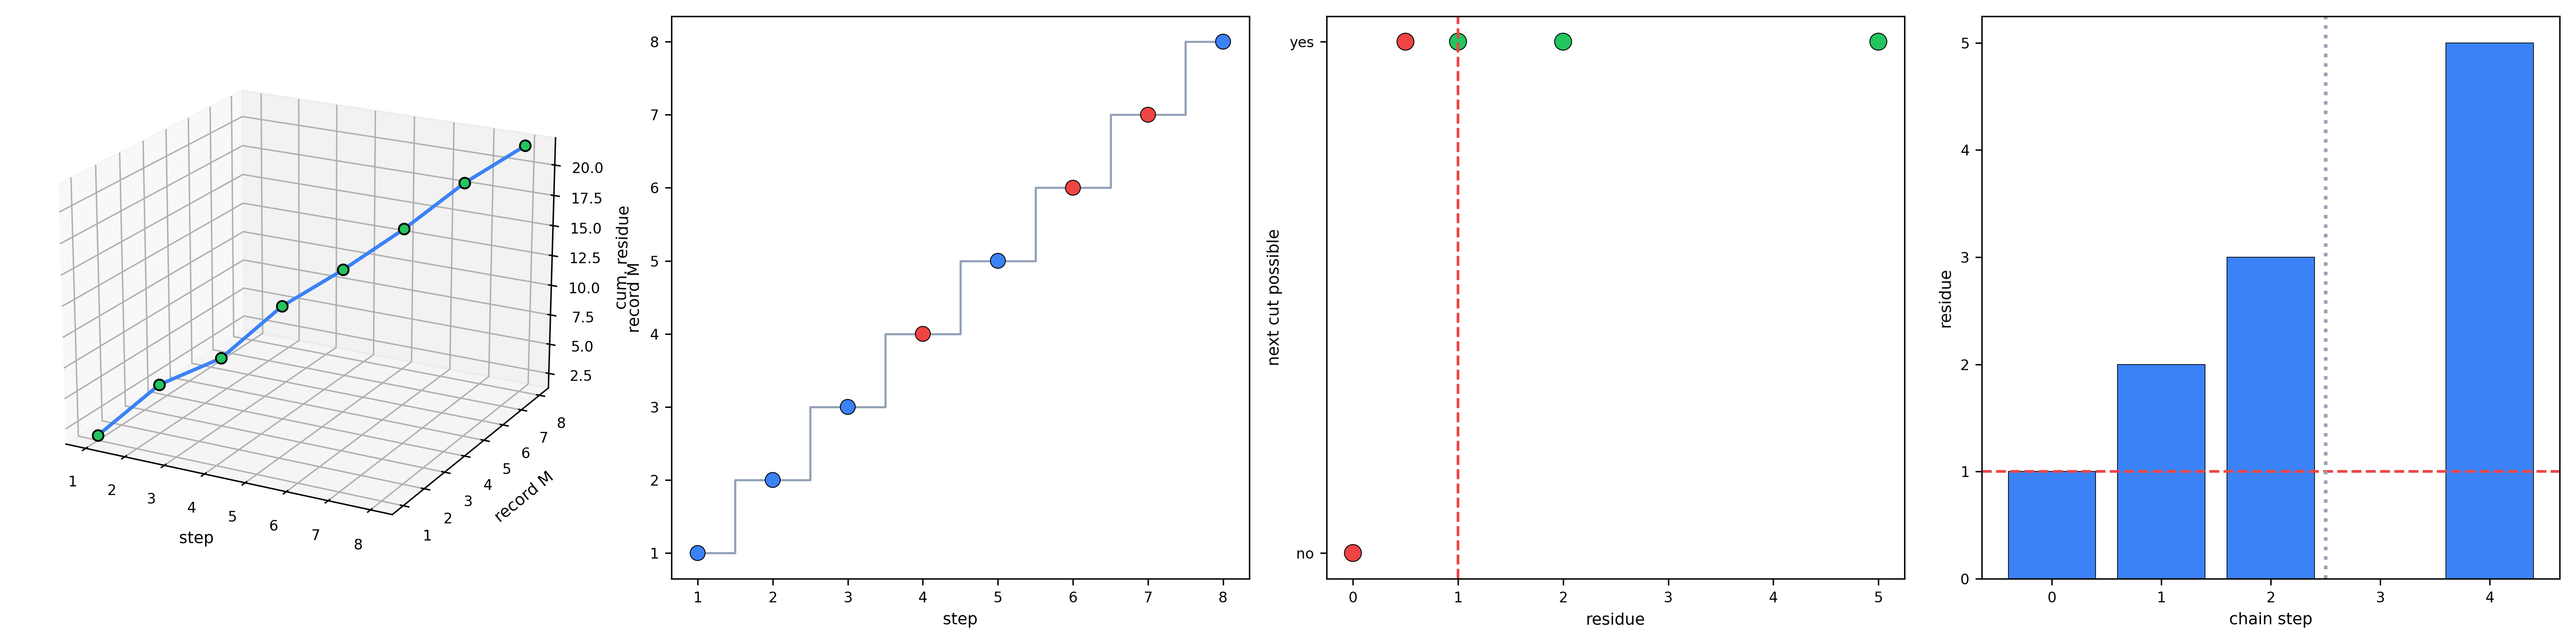
\includegraphics[width=\textwidth]{figures/panel_4_record_residue.png}
    \caption{\textbf{The Monotone Record and the Residue Propagator.}
    (\textbf{A})~Three-dimensional trajectory of a process in (step, committed record $M$, cumulative residue) space: the record climbs monotonically while the residue accumulates, the two coupled because each cut deposits a residue and increments the record (Theorem~\ref{thm:monotone}, Theorem~\ref{thm:propagator}).
    (\textbf{B})~Committed record $M$ versus step for an eight-event process; the staircase strictly increases, and the ``undo'' events (red points) increment the record exactly as forward cuts (blue) do---un-committing is itself a further cut, so the record never returns.
    (\textbf{C})~Whether a distinct next cut is possible (yes/no) versus the residue of the current cut; the transition occurs at residue zero, with points coloured green when the residue clears the floor $\beta$ (red dashed) and red otherwise. Residue $>0$ is necessary and sufficient for the next cut.
    (\textbf{D})~Residue at each step of a five-step chain, bars blue where the residue clears the floor and red where it would vanish; the dashed floor line $\beta$ and the halt marker (grey dotted) show the chain stopping exactly where a residue would fall below $\beta$---no residue, no next event.}
    \label{fig:panel_record_residue}
\end{figure*}

% ---------------------------------------------------------------------
\begin{figure*}[!htbp]
    \centering
    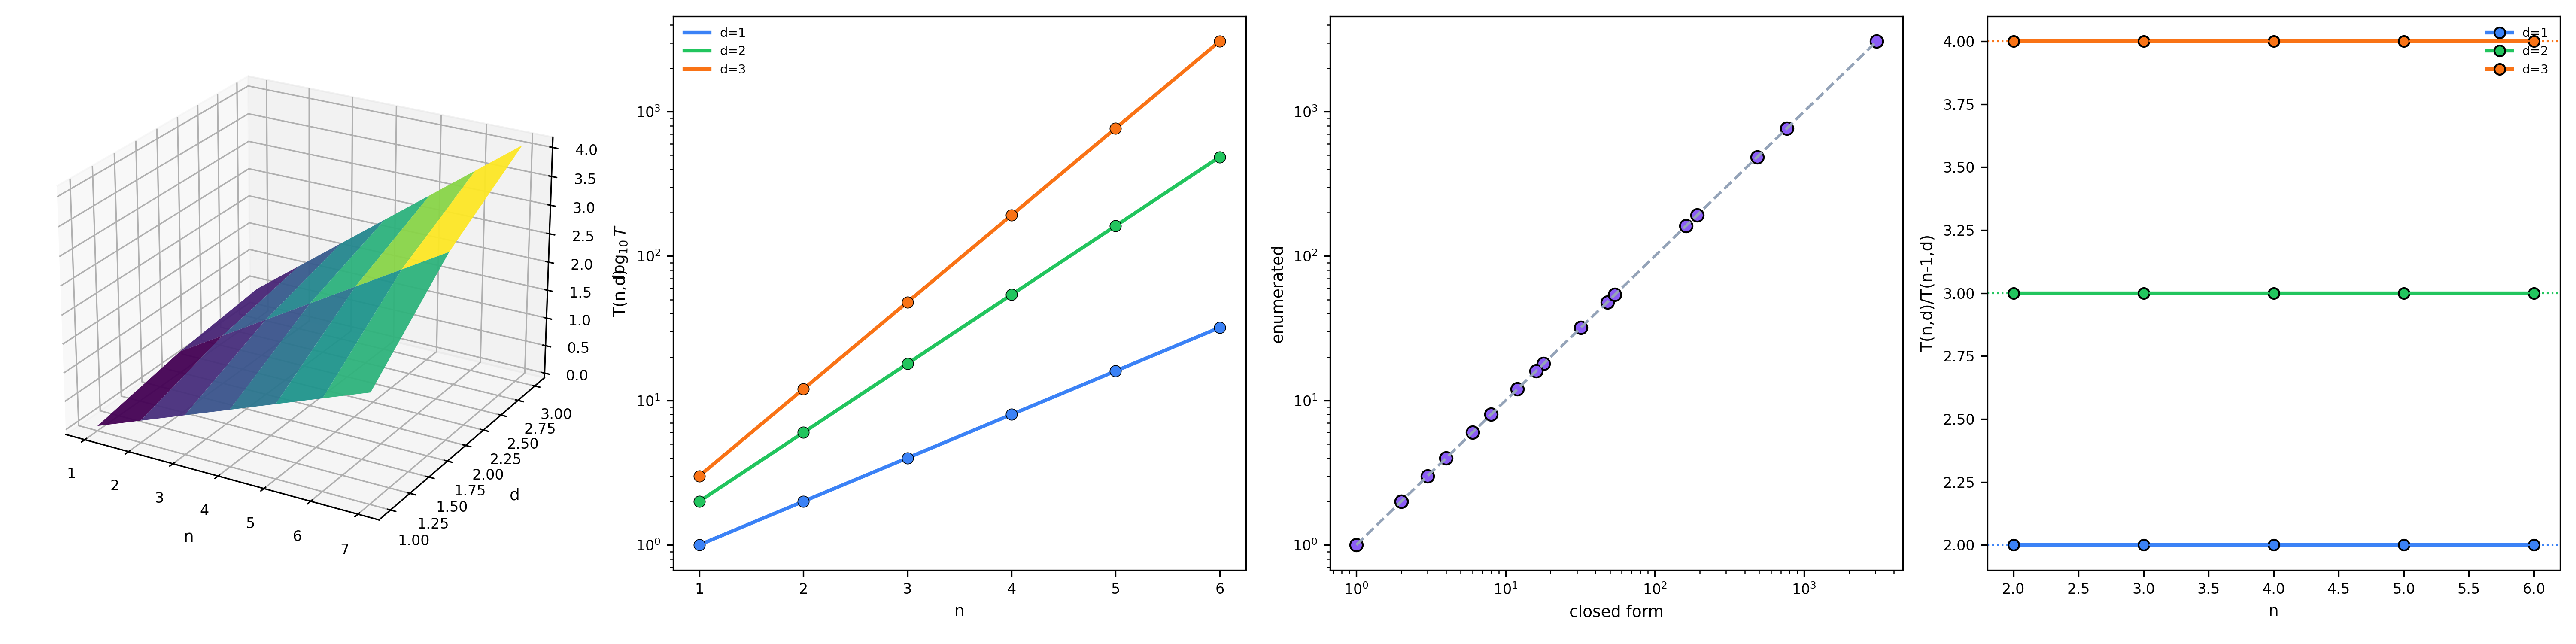
\includegraphics[width=\textwidth]{figures/panel_5_inflation.png}
    \caption{\textbf{Composition Inflation $T(n,d)=d(d+1)^{n-1}$.}
    (\textbf{A})~Three-dimensional surface of $\log_{10}T(n,d)$ over trajectory length $n$ and direction count $d$ (viridis); the surface rises steeply in $n$ and steepens with $d$, the exponential proliferation of distinguishable propagation trajectories with depth.
    (\textbf{B})~Trajectory count $T(n,d)$ on a logarithmic $y$-axis versus $n$ for $d=1,2,3$ (coloured lines), with directly enumerated counts (points) lying on the closed-form curves; enumeration and closed form agree exactly for every case computed.
    (\textbf{C})~Enumerated count versus closed form $d(d+1)^{n-1}$ on log--log axes; all points lie on the identity diagonal (grey dashed), the exact match of the brute-force enumeration to the formula.
    (\textbf{D})~Growth ratio $T(n,d)/T(n-1,d)$ versus $n$ for $d=1,2,3$ (coloured lines), each flat at its predicted value $d+1$ (dotted guides): the per-step branching factor is exactly $d+1$ (the $d$ moves plus the stay-option).}
    \label{fig:panel_inflation}
\end{figure*}

% ---------------------------------------------------------------------
\begin{figure*}[!htbp]
    \centering
    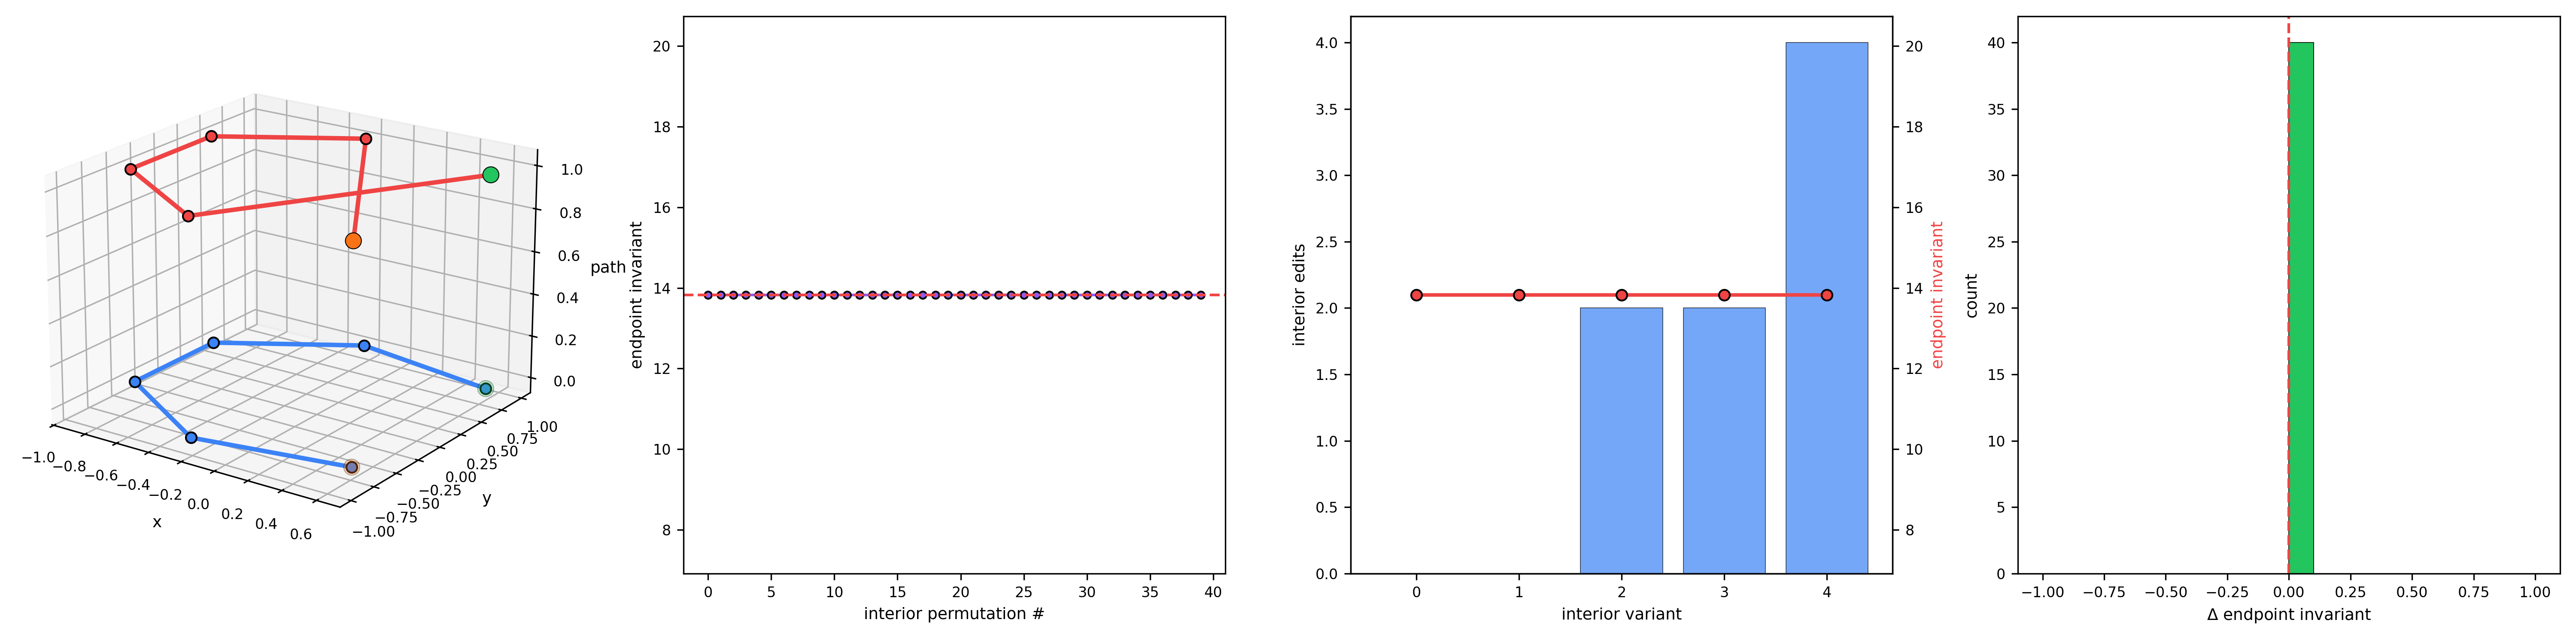
\includegraphics[width=\textwidth]{figures/panel_6_opacity.png}
    \caption{\textbf{Path Opacity: the Interior is Free.}
    (\textbf{A})~Three-dimensional rendering of two propagations sharing the same input (green) and output (orange) but distinct interior vertex orders, drawn on a circular item layout and lifted onto two path-index planes (blue and red). The two interiors differ while the endpoints coincide.
    (\textbf{B})~The endpoint invariant (the output's minimum-cut cost against the medium) across $40$ interior permutations; it is constant (points on the red dashed level), because the invariant depends only on the endpoints (Theorem~\ref{thm:path-opacity}).
    (\textbf{C})~Interior edit distance from a reference path (blue bars, left axis) growing across interior variants, against the endpoint invariant (red line, right axis) which stays flat: the interior may be edited arbitrarily without moving the endpoint invariant.
    (\textbf{D})~Distribution of the change $\Delta$ in the endpoint invariant across interior variants, a single spike at zero (red dashed): no interior rearrangement changes the endpoint invariant, so same-endpoint propagations are indistinguishable.}
    \label{fig:panel_opacity}
\end{figure*}

% ---------------------------------------------------------------------
\begin{figure*}[!htbp]
    \centering
    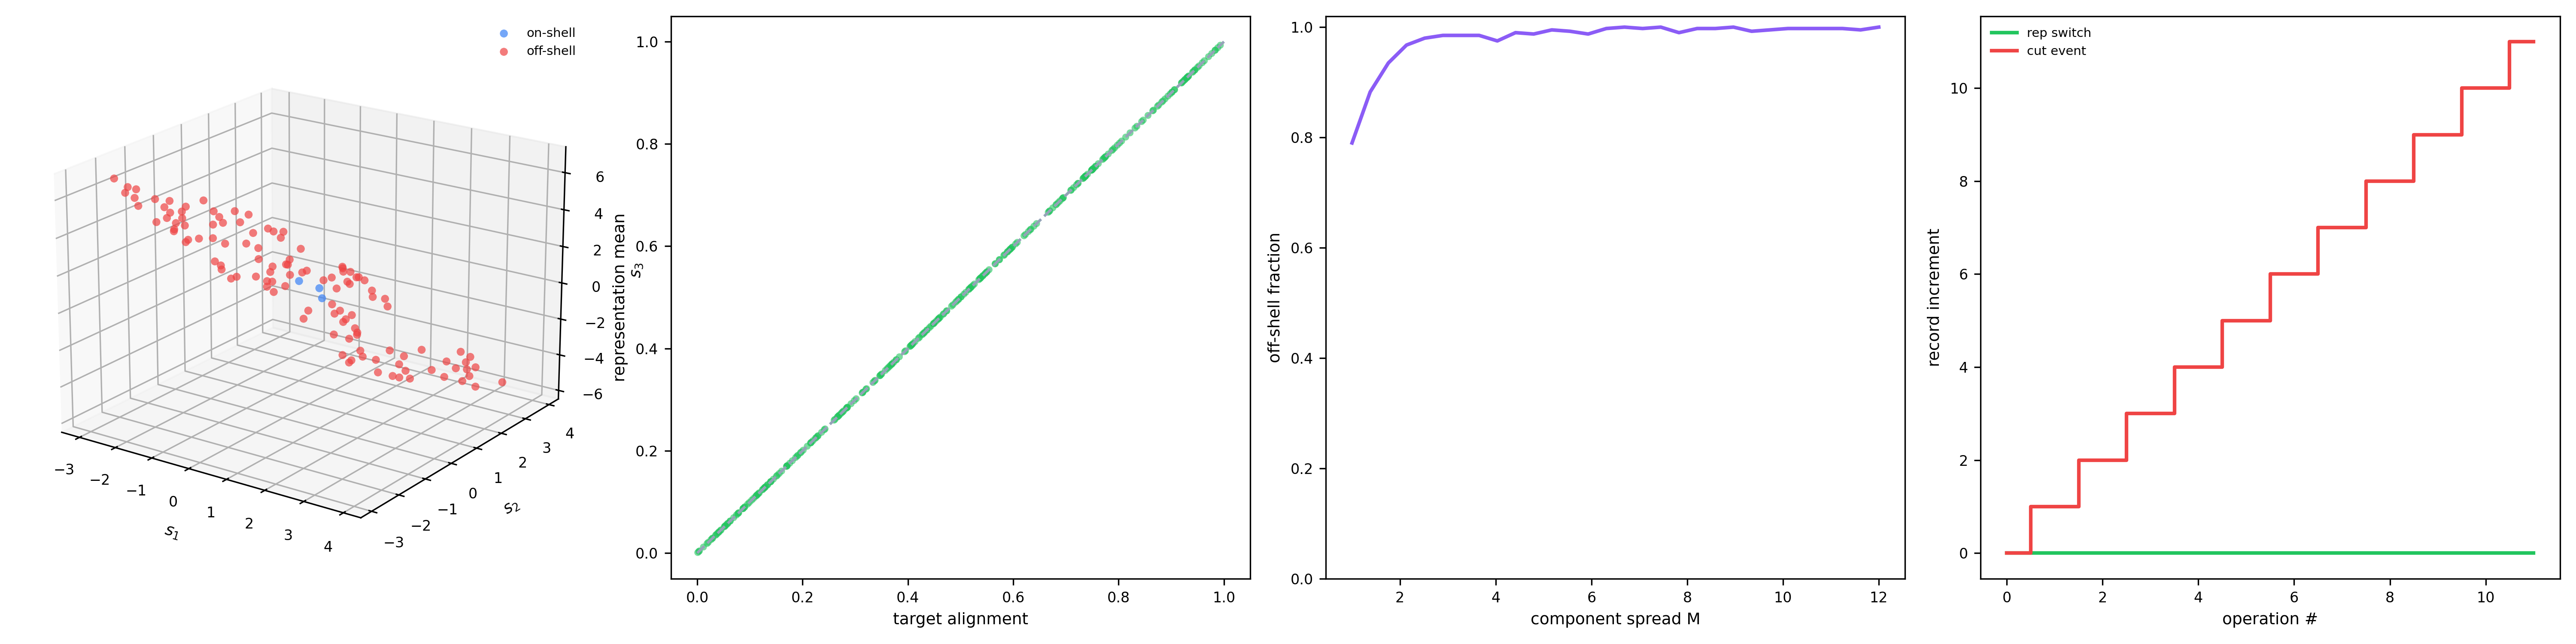
\includegraphics[width=\textwidth]{figures/panel_7_representation.png}
    \caption{\textbf{Representation Mobility and Mean Recovery.}
    (\textbf{A})~Three-dimensional scatter of $120$ three-component representations of a single item (alignment $0.5$) in $(s_1,s_2,s_3)$ space, coloured on-shell (blue, all components in $[0,1]$) or off-shell (red, some component outside): all lie on the mean-recovery plane $\tfrac13\sum s_j=0.5$, with off-shell components fully admissible (Theorem~\ref{thm:rep-mobility}).
    (\textbf{B})~Representation mean versus target alignment over $300$ random fibres and targets; every point lies on the diagonal (grey dashed): the component mean recovers the target exactly, whatever the individual components.
    (\textbf{C})~Off-shell fraction versus the component spread $M$; as the admissible spread grows the fraction of representations with an out-of-range component rises toward one, the freedom of the fibre to pass through ``impossible'' components while keeping the physical mean.
    (\textbf{D})~Record increment per operation: a representation switch (green) adds nothing to the committed record, while a cut event (red) increments it---switching representation commits no cut and leaves admissibility unchanged (Corollary~\ref{cor:mobility-required}).}
    \label{fig:panel_representation}
\end{figure*}

% ---------------------------------------------------------------------
\begin{figure*}[!htbp]
    \centering
    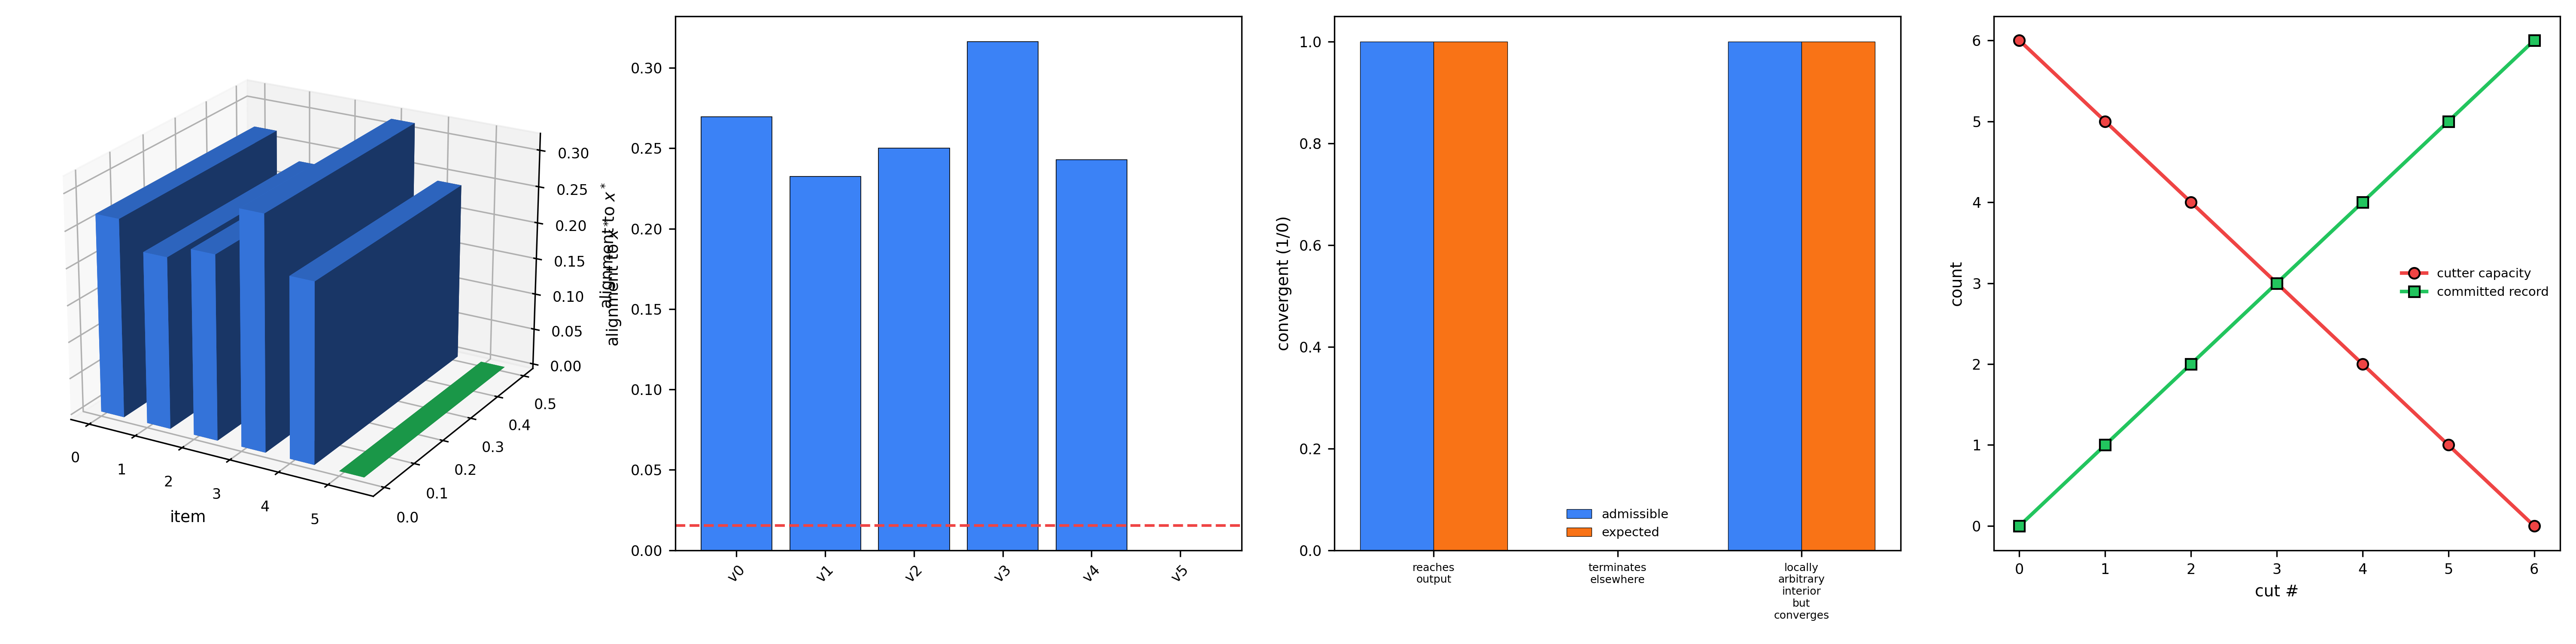
\includegraphics[width=\textwidth]{figures/panel_8_convergence_cut.png}
    \caption{\textbf{Convergence Admissibility and the One-Use Cut.}
    (\textbf{A})~Three-dimensional bar chart of each item's alignment to the output $x^{*}$ (cut cost to $x^{*}$ over total weight), the output bar green and the rest blue; only the output sits at the floor, the terminal accountable state of an admissible propagation.
    (\textbf{B})~Alignment to $x^{*}$ per item with the floor alignment $\beta/\Omega$ marked (red dashed); the output (green) alone reaches the floor, so a propagation is admissible exactly when it terminates there (Theorem~\ref{thm:admissibility}).
    (\textbf{C})~Convergence outcome for three cases---reaching the output, terminating elsewhere, and a locally arbitrary interior that nonetheless converges---with admissible (blue) and expected (orange) bars coinciding in each: admissibility tracks convergence to the output and nothing else, local steps being free.
    (\textbf{D})~The one-use, self-blunting cut: the cutter's uncommitted capacity (red) decreases by one per cut while the committed record (green) increases by one, the two crossing as capacity is spent. A cut commits once and blunts the cutter; the perfect repeatable traceless cut ($\beta=0$, record unchanged) cannot occur (Theorem~\ref{thm:one-use}, Theorem~\ref{thm:blunt}, Theorem~\ref{thm:no-perfect}).}
    \label{fig:panel_convergence_cut}
\end{figure*}
 or copy individually.
% =====================================================================

% ---------------------------------------------------------------------
\begin{figure*}[!htbp]
    \centering
    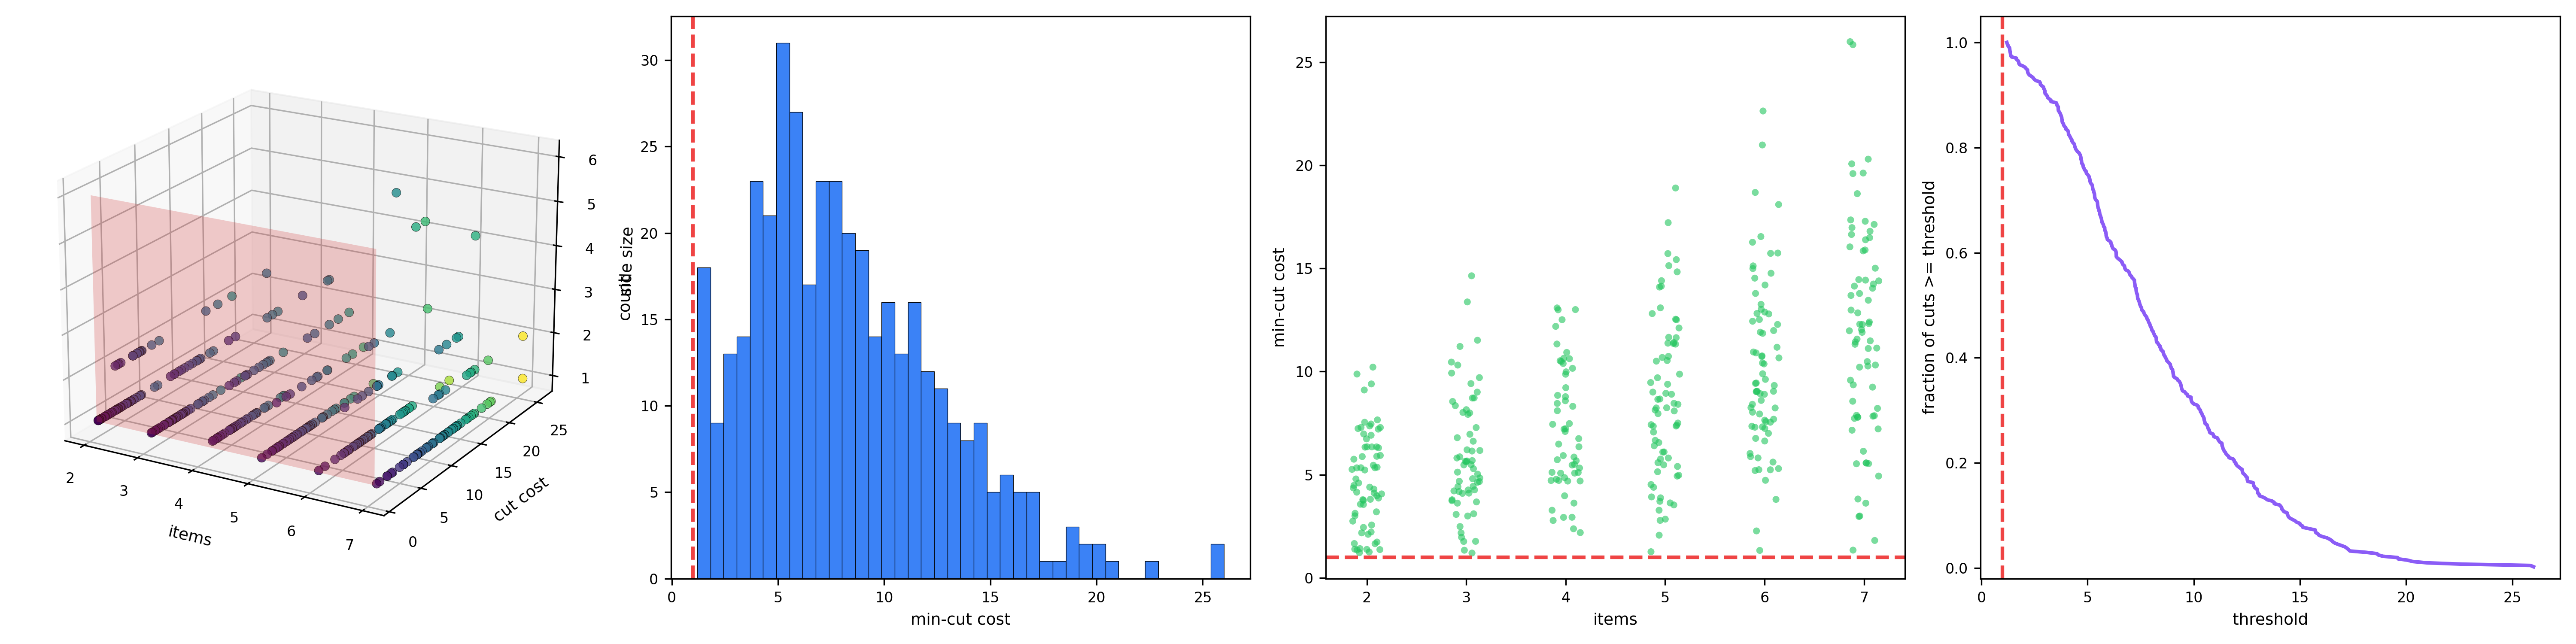
\includegraphics[width=\textwidth]{figures/panel_1_floor.png}
    \caption{\textbf{The Floor: Minimum Cuts over Random Contact Graphs.}
    (\textbf{A})~Three-dimensional scatter of $400$ random contact graphs in (number of items, minimum-cut cost, cut-side size) space, points coloured by cut cost (viridis), with the floor plane at cost $\beta$ drawn in red. Every point lies on or above the floor plane: no item is separated from the medium for less than $\beta$ (Theorem~\ref{thm:floor}).
    (\textbf{B})~Distribution of the exact minimum-cut costs (\texttt{networkx} max-flow) across the $400$ graphs, with the floor $\beta$ marked (red dashed). No mass falls below $\beta$, the absence of any sharp cut (Corollary~\ref{cor:no-sharp}).
    (\textbf{C})~Minimum-cut cost versus number of items (jittered) for all graphs; the entire cloud sits above the floor line $\beta$ (red dashed) independently of graph order, confirming the bound holds at every size.
    (\textbf{D})~Survival curve: the fraction of cuts with cost at least a given threshold, dropping from one only after the threshold passes $\beta$ (red dashed). The fraction at or above $\beta$ is unity---every one of the $300$ validated cuts clears the floor.}
    \label{fig:panel_floor}
\end{figure*}

% ---------------------------------------------------------------------
\begin{figure*}[!htbp]
    \centering
    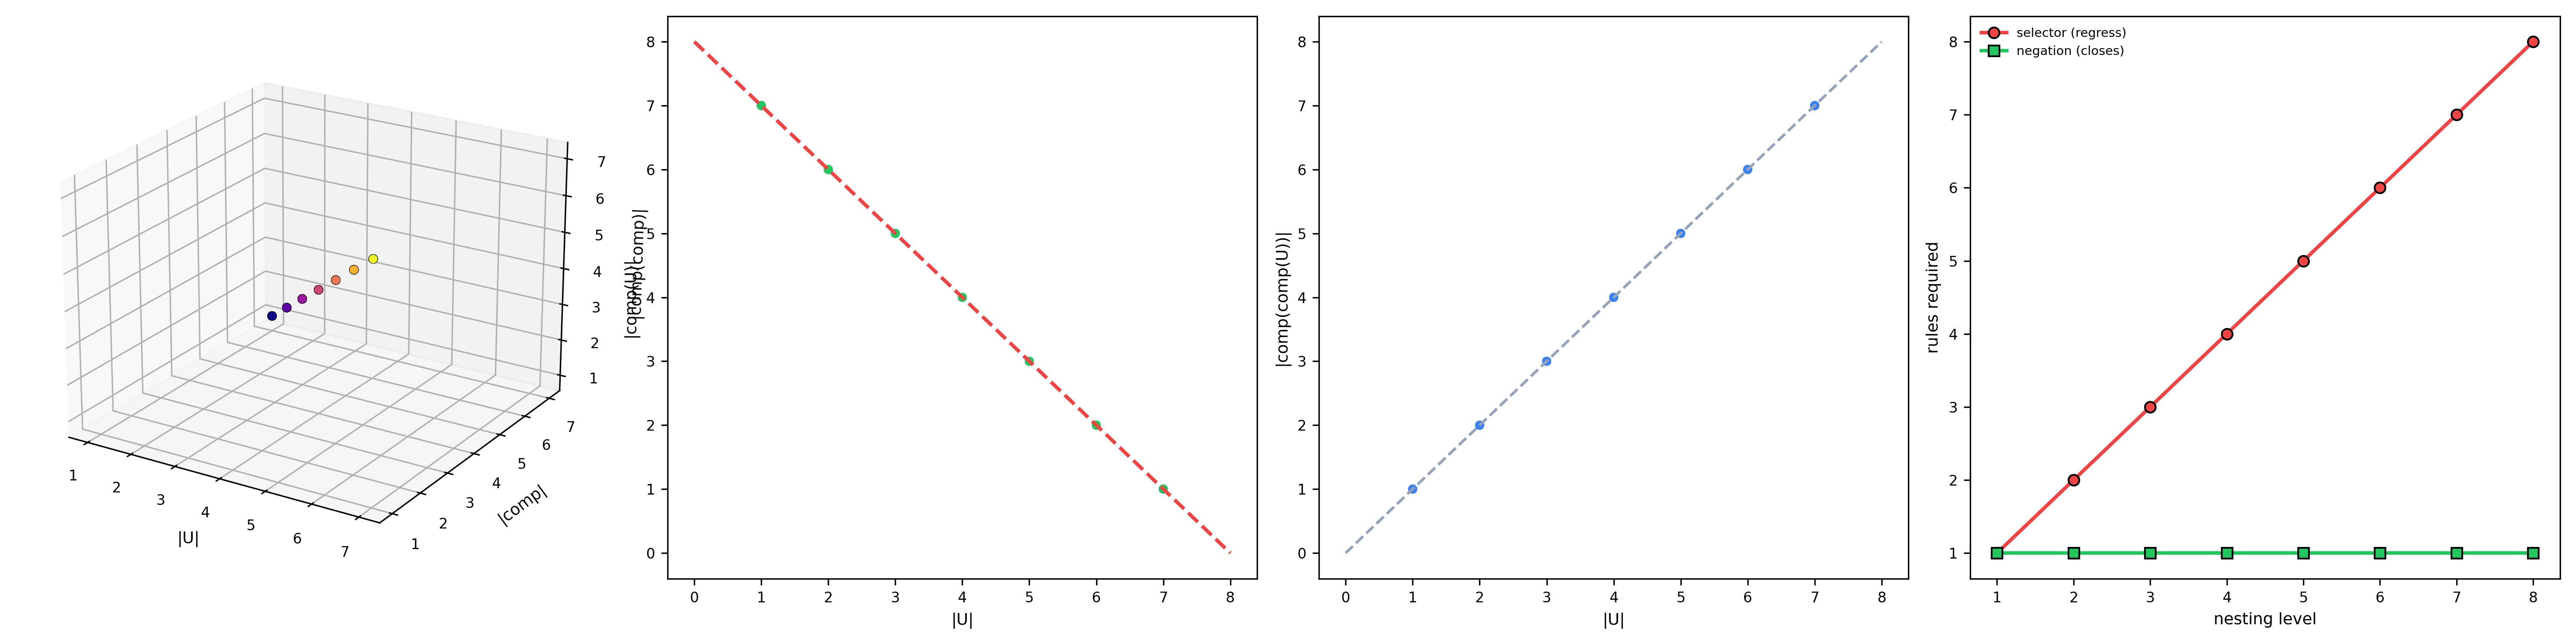
\includegraphics[width=\textwidth]{figures/panel_2_negation.png}
    \caption{\textbf{Individuation by Negation: the Complement Involution.}
    (\textbf{A})~Three-dimensional scatter of $200$ random subsets of an eight-element whole in $(|U|,\,|\co U|,\,|\co\co U|)$ space, coloured by $|U|$ (plasma). Every point satisfies $|\co\co U|=|U|$: double complementation returns the part, the involution underlying Theorem~\ref{thm:negation}.
    (\textbf{B})~Subset size $|U|$ versus complement size $|\co U|$; all points lie on the conservation line $|U|+|\co U|=8$ (red dashed): the complement is exactly ``the rest,'' fixed once the whole is given.
    (\textbf{C})~Double-complement size $|\co\co U|$ versus $|U|$ on the identity diagonal (grey dashed); the points coincide with the diagonal, so $\co$ is its own inverse and $\co U$ determines $U$ uniquely.
    (\textbf{D})~Rules required to fix a part as a function of nesting level: a positive (selector-based) rule regresses without bound (red), while negation closes at level one (green). The diverging red curve is the selector regress that Theorem~\ref{thm:negation} excludes; the flat green line is complementation, which needs only the whole.}
    \label{fig:panel_negation}
\end{figure*}

% ---------------------------------------------------------------------
\begin{figure*}[!htbp]
    \centering
    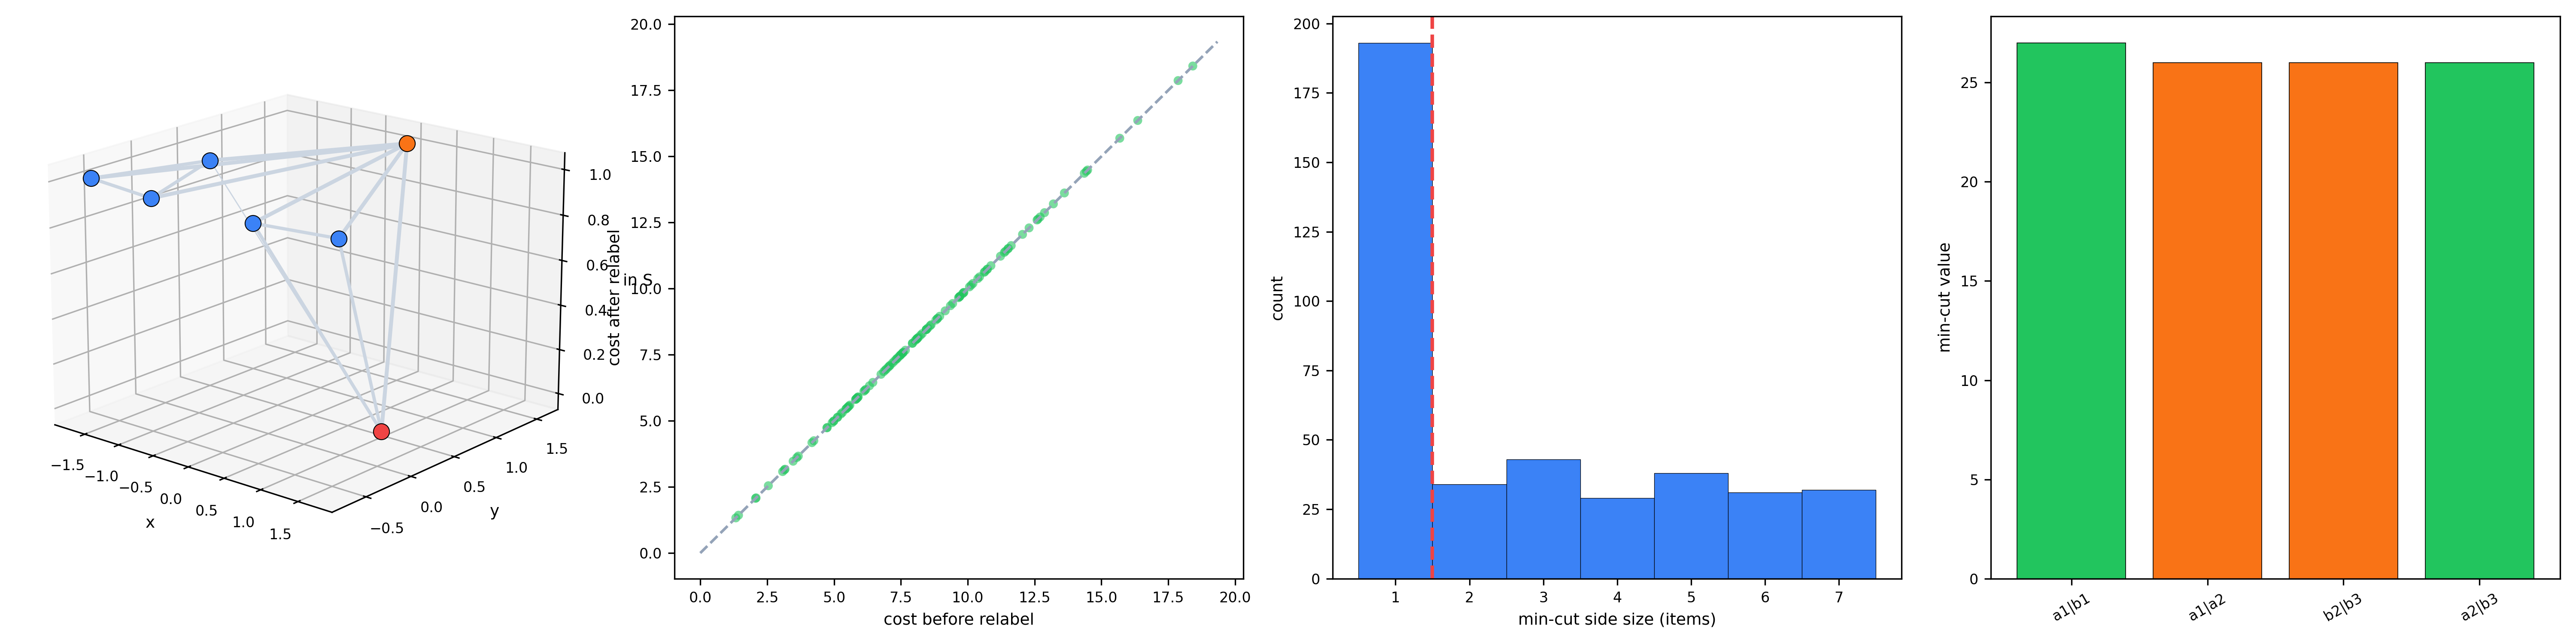
\includegraphics[width=\textwidth]{figures/panel_3_identity.png}
    \caption{\textbf{Identity as an Invariant Region, Never a Point.}
    (\textbf{A})~Three-dimensional rendering of the two-cluster contact graph: items (blue if on the source side $S$ of the minimum cut, red otherwise) and the medium (orange) at the origin, lifted on the vertical axis by cut membership, with edges drawn at width proportional to weight. The minimum cut places a multi-item set on the source side---identity is borne by a region, not a single vertex.
    (\textbf{B})~Minimum-cut cost before versus after a random relabelling (weighted isomorphism) of the items, over $120$ graphs; all points lie on the identity diagonal (grey dashed), so the cost is label-independent (Theorem~\ref{thm:invariant}).
    (\textbf{C})~Distribution of minimum-cut side sizes over $400$ random graphs; the mass lies predominantly above one item (the threshold at $1.5$, red dashed), the empirical content of ``the minimising side is in general not a singleton'' (Theorem~\ref{thm:region}).
    (\textbf{D})~Minimum-cut value for four different separated pairs in the two-cluster instance: the cluster-separating pairs (green) realise the cheap inter-cluster cut, while same-cluster pairs (orange) cost more, showing the cut value is a property of the partition, not of a chosen endpoint.}
    \label{fig:panel_identity}
\end{figure*}

% ---------------------------------------------------------------------
\begin{figure*}[!htbp]
    \centering
    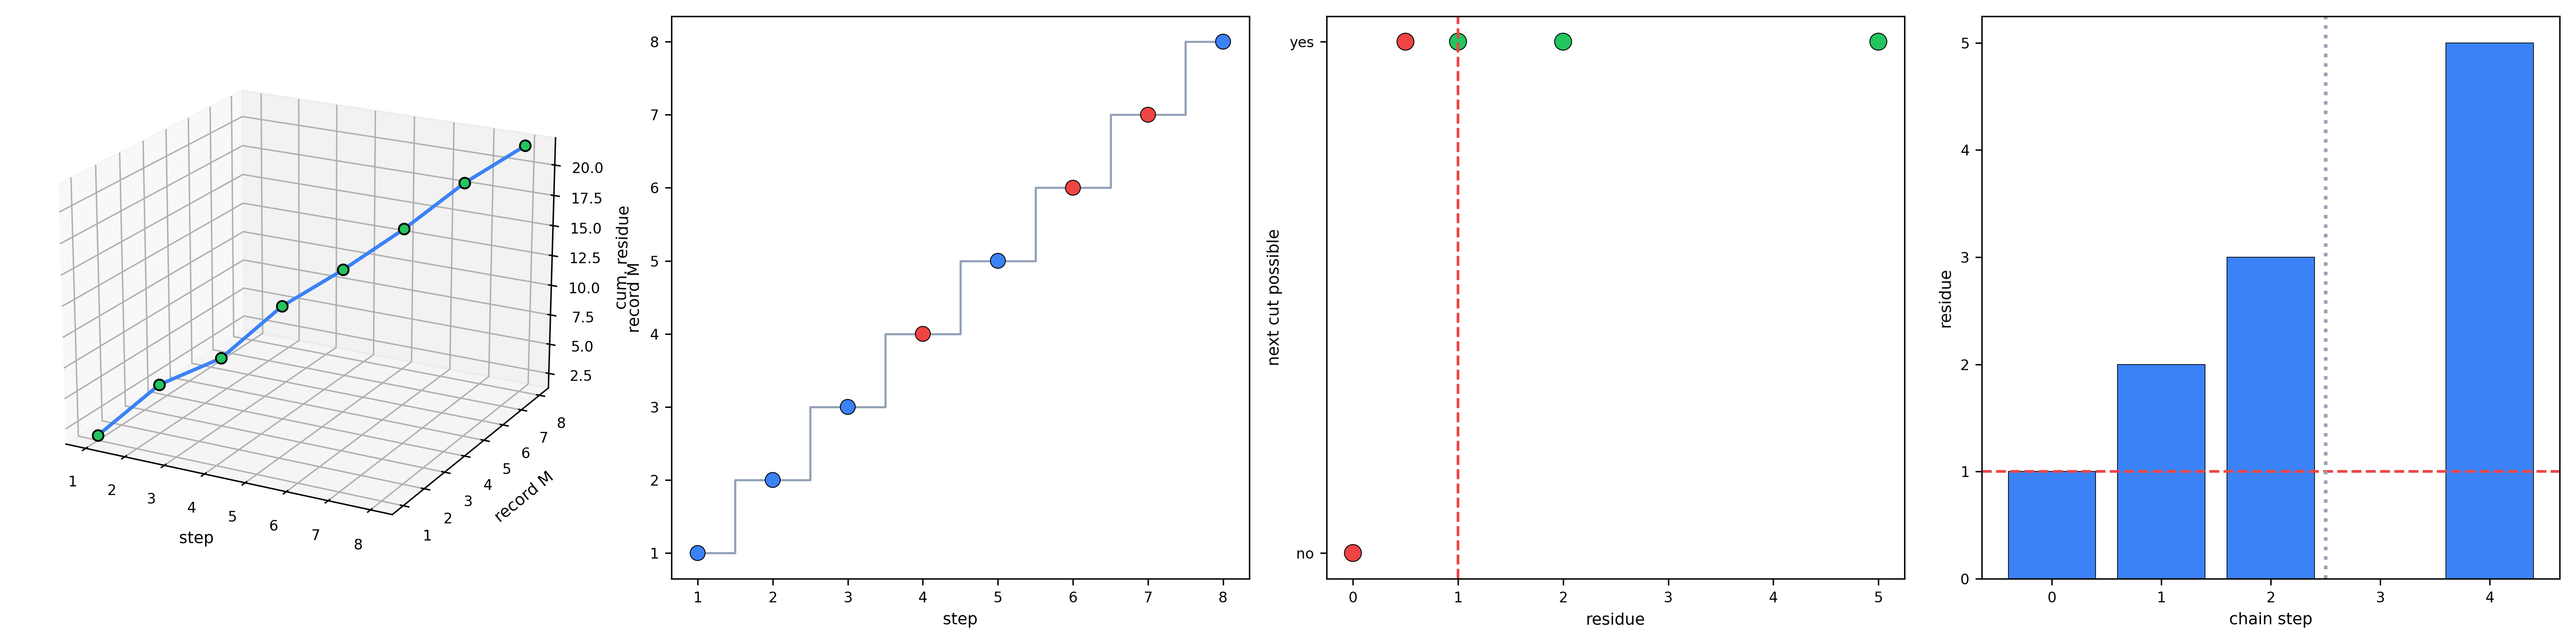
\includegraphics[width=\textwidth]{figures/panel_4_record_residue.png}
    \caption{\textbf{The Monotone Record and the Residue Propagator.}
    (\textbf{A})~Three-dimensional trajectory of a process in (step, committed record $M$, cumulative residue) space: the record climbs monotonically while the residue accumulates, the two coupled because each cut deposits a residue and increments the record (Theorem~\ref{thm:monotone}, Theorem~\ref{thm:propagator}).
    (\textbf{B})~Committed record $M$ versus step for an eight-event process; the staircase strictly increases, and the ``undo'' events (red points) increment the record exactly as forward cuts (blue) do---un-committing is itself a further cut, so the record never returns.
    (\textbf{C})~Whether a distinct next cut is possible (yes/no) versus the residue of the current cut; the transition occurs at residue zero, with points coloured green when the residue clears the floor $\beta$ (red dashed) and red otherwise. Residue $>0$ is necessary and sufficient for the next cut.
    (\textbf{D})~Residue at each step of a five-step chain, bars blue where the residue clears the floor and red where it would vanish; the dashed floor line $\beta$ and the halt marker (grey dotted) show the chain stopping exactly where a residue would fall below $\beta$---no residue, no next event.}
    \label{fig:panel_record_residue}
\end{figure*}

% ---------------------------------------------------------------------
\begin{figure*}[!htbp]
    \centering
    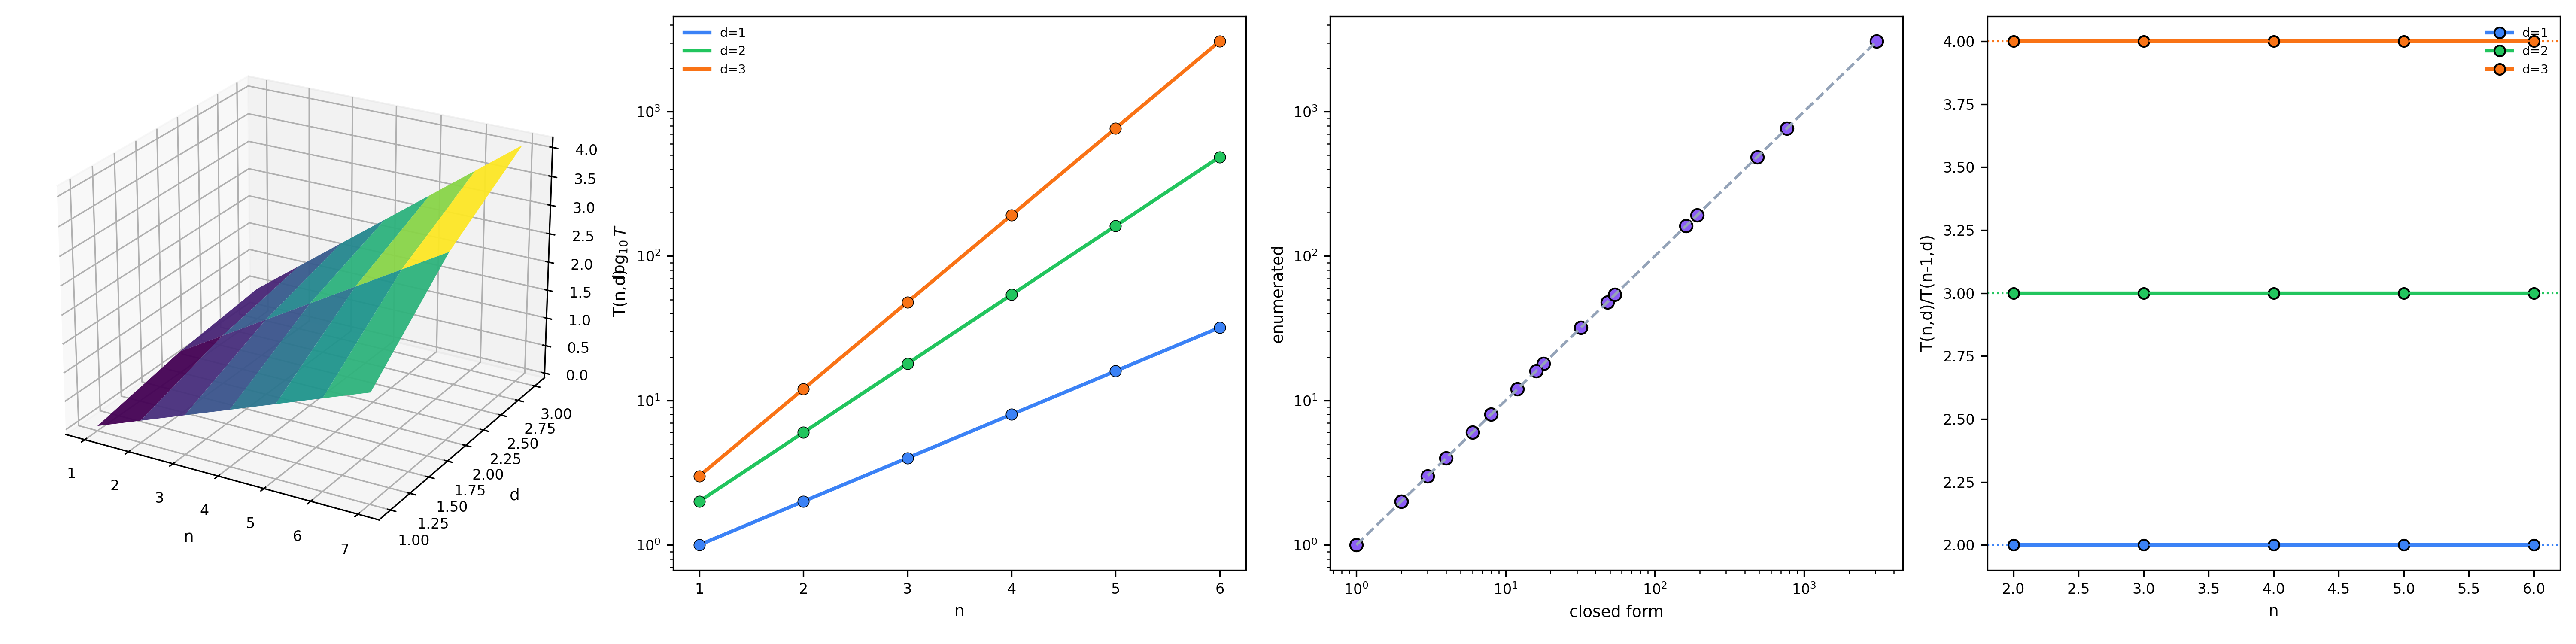
\includegraphics[width=\textwidth]{figures/panel_5_inflation.png}
    \caption{\textbf{Composition Inflation $T(n,d)=d(d+1)^{n-1}$.}
    (\textbf{A})~Three-dimensional surface of $\log_{10}T(n,d)$ over trajectory length $n$ and direction count $d$ (viridis); the surface rises steeply in $n$ and steepens with $d$, the exponential proliferation of distinguishable propagation trajectories with depth.
    (\textbf{B})~Trajectory count $T(n,d)$ on a logarithmic $y$-axis versus $n$ for $d=1,2,3$ (coloured lines), with directly enumerated counts (points) lying on the closed-form curves; enumeration and closed form agree exactly for every case computed.
    (\textbf{C})~Enumerated count versus closed form $d(d+1)^{n-1}$ on log--log axes; all points lie on the identity diagonal (grey dashed), the exact match of the brute-force enumeration to the formula.
    (\textbf{D})~Growth ratio $T(n,d)/T(n-1,d)$ versus $n$ for $d=1,2,3$ (coloured lines), each flat at its predicted value $d+1$ (dotted guides): the per-step branching factor is exactly $d+1$ (the $d$ moves plus the stay-option).}
    \label{fig:panel_inflation}
\end{figure*}

% ---------------------------------------------------------------------
\begin{figure*}[!htbp]
    \centering
    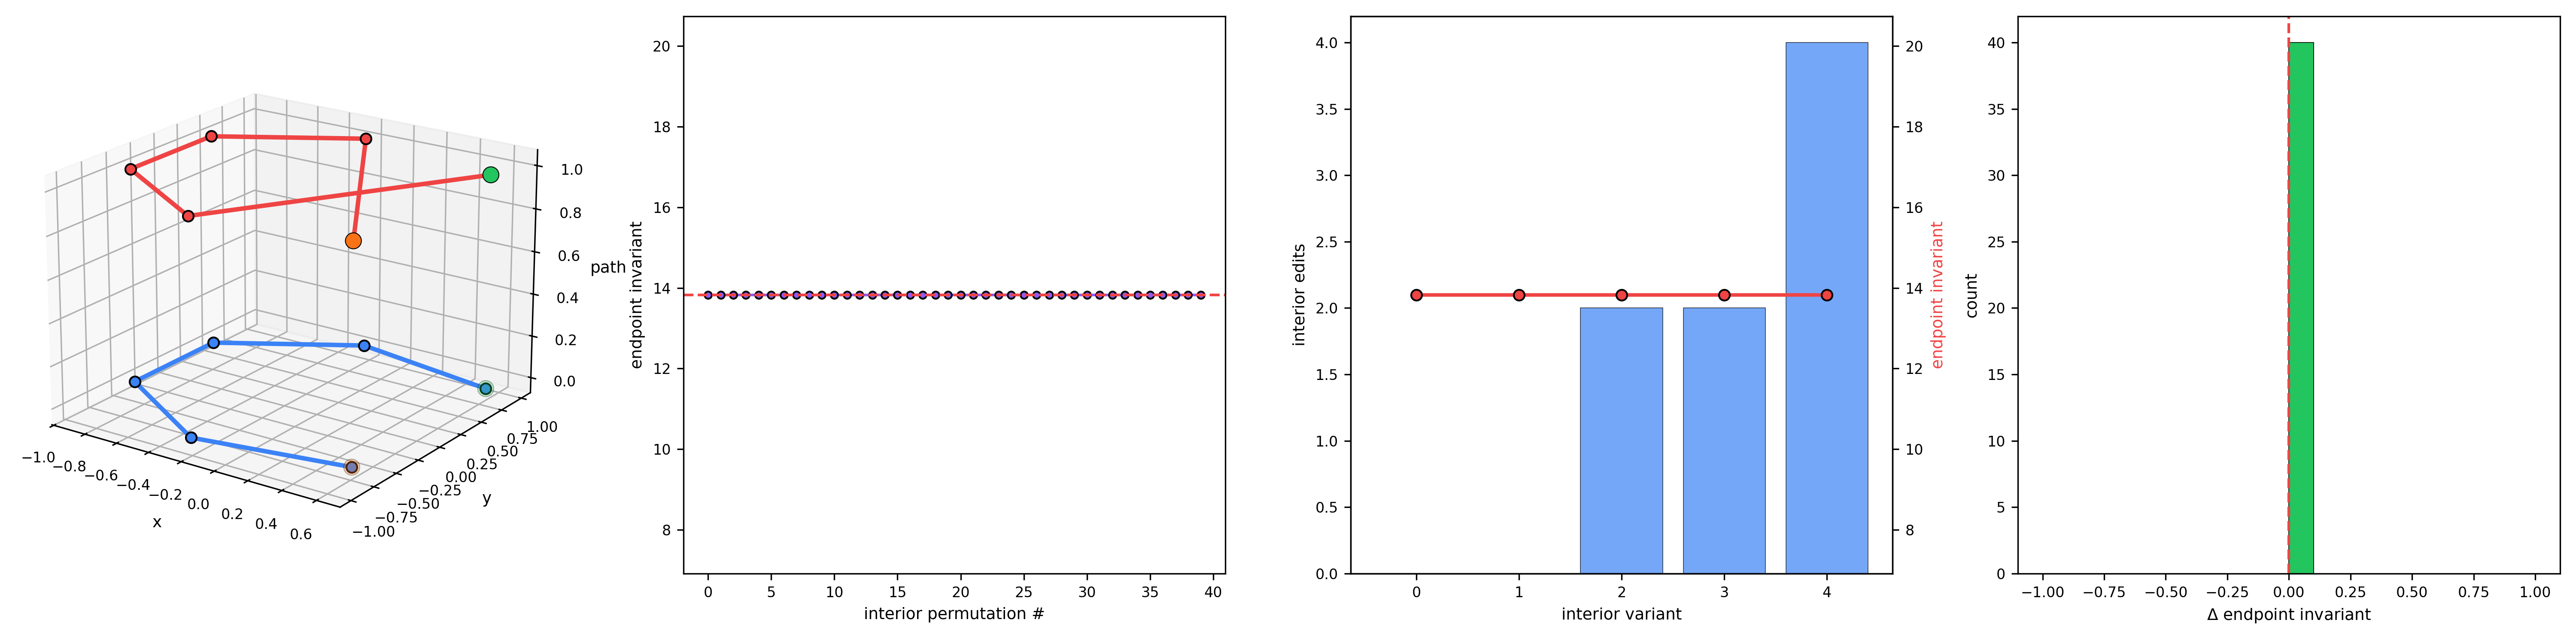
\includegraphics[width=\textwidth]{figures/panel_6_opacity.png}
    \caption{\textbf{Path Opacity: the Interior is Free.}
    (\textbf{A})~Three-dimensional rendering of two propagations sharing the same input (green) and output (orange) but distinct interior vertex orders, drawn on a circular item layout and lifted onto two path-index planes (blue and red). The two interiors differ while the endpoints coincide.
    (\textbf{B})~The endpoint invariant (the output's minimum-cut cost against the medium) across $40$ interior permutations; it is constant (points on the red dashed level), because the invariant depends only on the endpoints (Theorem~\ref{thm:path-opacity}).
    (\textbf{C})~Interior edit distance from a reference path (blue bars, left axis) growing across interior variants, against the endpoint invariant (red line, right axis) which stays flat: the interior may be edited arbitrarily without moving the endpoint invariant.
    (\textbf{D})~Distribution of the change $\Delta$ in the endpoint invariant across interior variants, a single spike at zero (red dashed): no interior rearrangement changes the endpoint invariant, so same-endpoint propagations are indistinguishable.}
    \label{fig:panel_opacity}
\end{figure*}

% ---------------------------------------------------------------------
\begin{figure*}[!htbp]
    \centering
    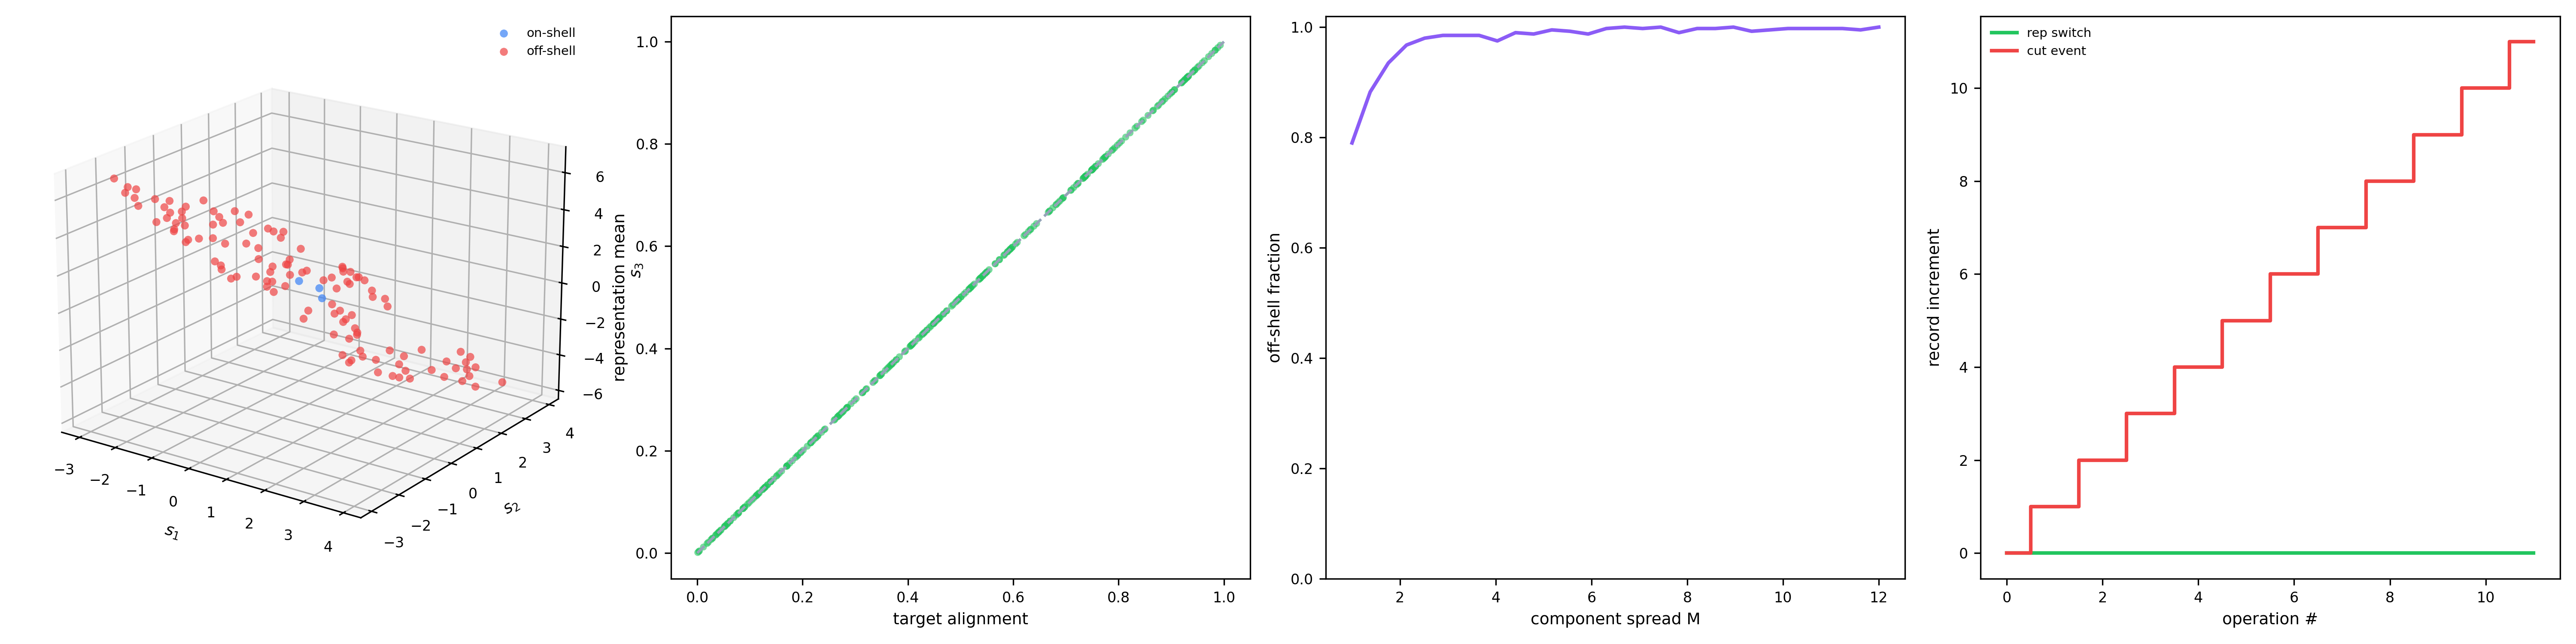
\includegraphics[width=\textwidth]{figures/panel_7_representation.png}
    \caption{\textbf{Representation Mobility and Mean Recovery.}
    (\textbf{A})~Three-dimensional scatter of $120$ three-component representations of a single item (alignment $0.5$) in $(s_1,s_2,s_3)$ space, coloured on-shell (blue, all components in $[0,1]$) or off-shell (red, some component outside): all lie on the mean-recovery plane $\tfrac13\sum s_j=0.5$, with off-shell components fully admissible (Theorem~\ref{thm:rep-mobility}).
    (\textbf{B})~Representation mean versus target alignment over $300$ random fibres and targets; every point lies on the diagonal (grey dashed): the component mean recovers the target exactly, whatever the individual components.
    (\textbf{C})~Off-shell fraction versus the component spread $M$; as the admissible spread grows the fraction of representations with an out-of-range component rises toward one, the freedom of the fibre to pass through ``impossible'' components while keeping the physical mean.
    (\textbf{D})~Record increment per operation: a representation switch (green) adds nothing to the committed record, while a cut event (red) increments it---switching representation commits no cut and leaves admissibility unchanged (Corollary~\ref{cor:mobility-required}).}
    \label{fig:panel_representation}
\end{figure*}

% ---------------------------------------------------------------------
\begin{figure*}[!htbp]
    \centering
    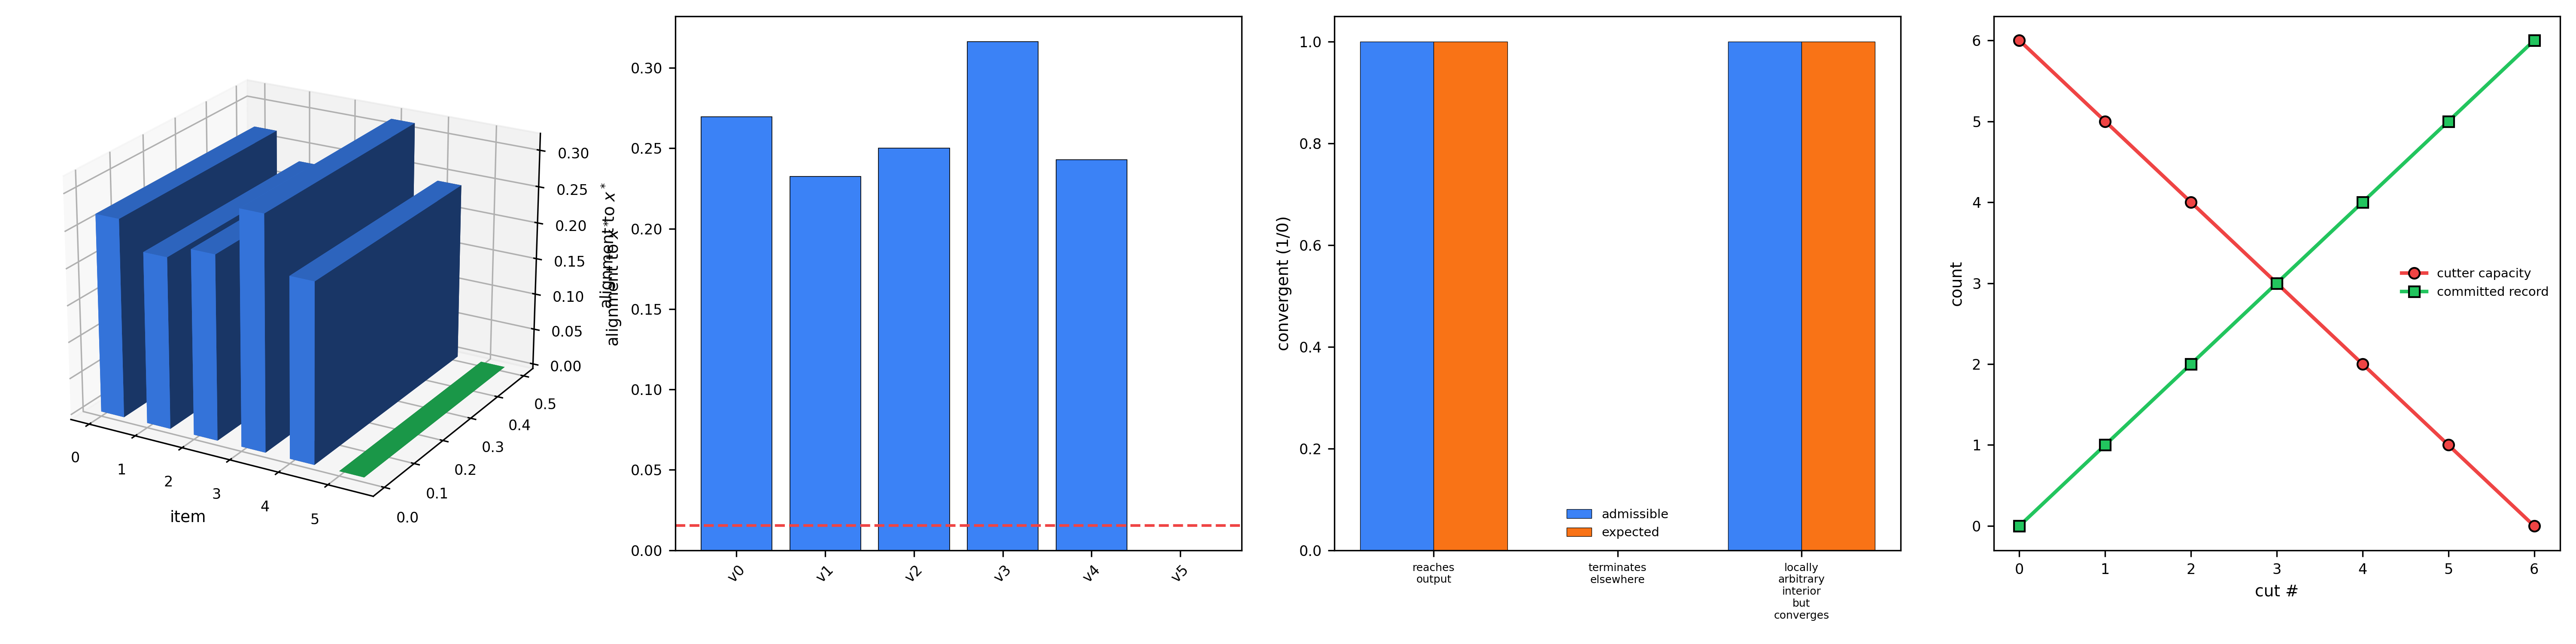
\includegraphics[width=\textwidth]{figures/panel_8_convergence_cut.png}
    \caption{\textbf{Convergence Admissibility and the One-Use Cut.}
    (\textbf{A})~Three-dimensional bar chart of each item's alignment to the output $x^{*}$ (cut cost to $x^{*}$ over total weight), the output bar green and the rest blue; only the output sits at the floor, the terminal accountable state of an admissible propagation.
    (\textbf{B})~Alignment to $x^{*}$ per item with the floor alignment $\beta/\Omega$ marked (red dashed); the output (green) alone reaches the floor, so a propagation is admissible exactly when it terminates there (Theorem~\ref{thm:admissibility}).
    (\textbf{C})~Convergence outcome for three cases---reaching the output, terminating elsewhere, and a locally arbitrary interior that nonetheless converges---with admissible (blue) and expected (orange) bars coinciding in each: admissibility tracks convergence to the output and nothing else, local steps being free.
    (\textbf{D})~The one-use, self-blunting cut: the cutter's uncommitted capacity (red) decreases by one per cut while the committed record (green) increases by one, the two crossing as capacity is spent. A cut commits once and blunts the cutter; the perfect repeatable traceless cut ($\beta=0$, record unchanged) cannot occur (Theorem~\ref{thm:one-use}, Theorem~\ref{thm:blunt}, Theorem~\ref{thm:no-perfect}).}
    \label{fig:panel_convergence_cut}
\end{figure*}
